\chapter{Multivariable Integral} \label{mi:chapter}


%%%%%%%%%%%%%%%%%%%%%%%%%%%%%%%%%%%%%%%%%%%%%%%%%%%%%%%%%%%%%%%%%%%%%%%%%%%%%%

\section{Riemann integral over rectangles}
\label{sec:rirect}

\sectionnotes{2--3 lectures}

As in \chapterref{int:chapter}, we define the Riemann integral using the Darboux
upper and lower integrals.  The ideas in this section are very similar to
integration in one dimension.  The complication is mostly notational.
The differences between one and several dimensions will grow more pronounced
in the sections following.

\subsection{Rectangles and partitions}

\begin{defn}
Let $(a_1,a_2,\ldots,a_n)$ and
$(b_1,b_2,\ldots,b_n)$ be such that $a_k \leq b_k$ for all $k$.
The set
$[a_1,b_1] \times
[a_2,b_2] \times \cdots \times
[a_n,b_n]$ is called a \emph{\myindex{closed rectangle}}\index{rectangle}.
In this setting it is sometimes useful to allow $a_k = b_k$, in which case we 
think of $[a_k,b_k] = \{ a_k \}$ as usual.
If $a_k < b_k$ for all $k$, then the set
$(a_1,b_1) \times
(a_2,b_2) \times \cdots \times
(a_n,b_n)$ is called an \emph{\myindex{open rectangle}}.

For an open or closed rectangle
$R \coloneqq [a_1,b_1] \times
[a_2,b_2] \times \cdots \times
[a_n,b_n] \subset \R^n$
or
$R \coloneqq (a_1,b_1) \times
(a_2,b_2) \times \cdots \times
(a_n,b_n) \subset \R^n$,
we define the
\emph{$n$-dimensional volume}%
\index{n-dimensional volume@$n$-dimensional volume!rectangles}%
\index{volume of rectangles} by
\glsadd{not:ndimvolume}
\begin{equation*}
V(R) \coloneqq
(b_1-a_1)
(b_2-a_2)
\cdots
(b_n-a_n) .
\end{equation*}

A \emph{\myindex{partition}} $P$ of the closed rectangle
$R = [a_1,b_1] \times
[a_2,b_2] \times \cdots \times
[a_n,b_n]$
is given by
partitions $P_1,P_2,\ldots,P_n$ of the intervals
$[a_1,b_1], [a_2,b_2],\ldots, [a_n,b_n]$.
We write $P=(P_1,P_2,\ldots,P_n)$.
That is, for every $k=1,2,\ldots,n$ there is an integer $\ell_k$ and
a finite set of numbers
$P_k = \{ x_{k,0},x_{k,1},x_{k,2},\ldots,x_{k,\ell_k} \}$ such that
\begin{equation*}
a_k = x_{k,0} < x_{k,1} < x_{k,2} < \cdots < x_{k,{\ell_k}-1} < x_{k,\ell_k} = b_k .
\end{equation*}
Picking a set of $n$ integers $j_1,j_2,\ldots,j_n$ where
$j_k \in \{ 1,2,\ldots,\ell_k \}$ we get
the
\emph{\myindex{subrectangle}}
\begin{equation*}
[x_{1,j_1-1}~,~ x_{1,j_1}]
\times
[x_{2,j_2-1}~,~ x_{2,j_2}]
\times
\cdots
\times
[x_{n,j_n-1}~,~ x_{n,j_n}] .
\end{equation*}
We order the subrectangles somehow and
we say $\{R_1,R_2,\ldots,R_N\}$ are the subrectangles corresponding
to the partition $P$ of $R$, or more simply, subrectangles of
$P$.
In other words, we subdivided the original rectangle into many smaller
subrectangles.  See \figureref{mv:figrect}.

\begin{myfigureht}
\subimport*{figures/}{figrect.pdf_t}
\caption{Example partition of a rectangle in $\R^2$.  The order of the
subrectangles is not important.\label{mv:figrect}}
\end{myfigureht}

Let $R \subset \R^n$ be a closed rectangle and
let $f \colon R \to \R$ be a bounded function.  Let $P$ be a partition of
$R$ with $N$ subrectangles $R_1,R_2,\ldots,R_N$.
Define
\glsadd{not:lowerdarbouxsum}
\glsadd{not:upperdarbouxsum}
\begin{align*}
& m_i \coloneqq \inf \bigl\{ f(x) : x \in R_i \bigr\} , & 
& M_i \coloneqq \sup \bigl\{ f(x) : x \in R_i \bigr\} , \\
& L(P,f) \coloneqq
\sum_{i=1}^N m_i V(R_i) , &
& U(P,f) \coloneqq
\sum_{i=1}^N M_i V(R_i) .
\end{align*}
We call $L(P,f)$ the \emph{\myindex{lower Darboux sum}} and
$U(P,f)$ the \emph{\myindex{upper Darboux sum}}\index{Darboux sum}.
\end{defn}

To see the relationship to the $\Delta$ notation from the one-variable
definition, note that when
\begin{equation*}
R_i = [x_{1,j_1-1}~,~ x_{1,j_1}]
\times
[x_{2,j_2-1}~,~ x_{2,j_2}]
\times
\cdots
\times
[x_{n,j_n-1}~,~ x_{n,j_n}] ,
\end{equation*}
then
\begin{equation*}
V(R_i)
=
(x_{1,j_1}-x_{1,j_1-1})
(x_{2,j_2}-x_{2,j_2-1})
\cdots
(x_{n,j_n}-x_{n,j_n-1})
= 
\Delta x_{1,j_1}
\Delta x_{2,j_2}
\cdots
\Delta x_{n,j_n} .
\end{equation*}
It is not difficult to see (left to reader) that
the subrectangles of $P$ cover our original $R$, and their
volumes sum to that of $R$.  That is,
\begin{equation*}
R= \bigcup_{k=1}^N R_k , \qquad \text{and} \qquad
V(R) = \sum_{k=1}^N V(R_k).
\end{equation*}

The indexing in the definition may be complicated, but fortunately we
do not need to go back directly to the definition often.

\begin{prop} \label{mv:sumulbound:prop}
Suppose $R \subset \R^n$ is a closed rectangle
and $f \colon R \to \R$ is a bounded function.  Let $m, M \in \R$ be 
such that for all $x \in R$, we have $m \leq f(x) \leq M$.  Then for every partition
$P$ of~$R$,
\begin{equation*}
m \, V(R) \leq
L(P,f) \leq U(P,f)
\leq M\, V(R) .
\end{equation*}
\end{prop}

\begin{proof}
Let $P$ be a partition of $R$.  For all $i$, we have
$m \leq m_i \leq M_i \leq M$.  Also $\sum_{i=1}^N V(R_i) = V(R)$.  Therefore,
\begin{multline*}
m \, V(R) =
m \left( \sum_{i=1}^N V(R_i) \right)
=
\sum_{i=1}^N m \, V(R_i)
\leq
\sum_{i=1}^N m_i \, V(R_i)
\leq
\\
\leq
\sum_{i=1}^N M_i \, V(R_i)
\leq
\sum_{i=1}^N M \,V(R_i)
=
M \left( \sum_{i=1}^N V(R_i) \right)
=
M \,V(R) .  \qedhere
\end{multline*}
\end{proof}

\subsection{Upper and lower integrals}

By \propref{mv:sumulbound:prop}, the set of upper and lower Darboux sums are bounded sets and we can take
their infima and suprema.  As in one variable, we make the following definition.

\begin{defn}
Let $f \colon R \to \R$ be a bounded function on a closed rectangle $R \subset
\R^n$.
Define
\glsadd{not:lowerdarbouxR}
\glsadd{not:upperdarbouxR}
\begin{equation*}
\underline{\int_R} f
\coloneqq \sup \, \bigl\{ L(P,f) : P \text{ a partition of } R \bigr\} , 
\qquad
\overline{\int_R} f
\coloneqq \inf \, \bigl\{ U(P,f) : P \text{ a partition of } R \bigr\} .
\end{equation*}
We call $\underline{\int}$ the
\emph{\myindex{lower Darboux integral}}\index{Darboux integral} and
$\overline{\int}$ the \emph{\myindex{upper Darboux integral}}.
\end{defn}

And as in one dimension, we define refinements of partitions.

\begin{defn}
Let $R \subset \R^n$ be a closed rectangle.
Let $P = ( P_1, P_2, \ldots, P_n )$
and $\widetilde{P} = ( \widetilde{P}_1, \widetilde{P}_2, \ldots, \widetilde{P}_n )$
be partitions of $R$.  We say $\widetilde{P}$ a
\emph{refinement}\index{refinement of a partition} of $P$
if, as sets, $P_k \subset \widetilde{P}_k$ for all $k = 1,2,\ldots,n$.
\end{defn}

If $\widetilde{P}$ is a refinement of $P$,
then subrectangles of $P$ are unions of subrectangles of $\widetilde{P}$.
Simply put, in a refinement, we take the subrectangles of $P$,
and we cut them into smaller subrectangles and call that $\widetilde{P}$.
See \figureref{mv:figrectpart}.

\begin{myfigureht}
\subimport*{figures/}{figrectpart.pdf_t}
\caption{Example refinement of the partition from \figureref{mv:figrect}.
New \myquote{cuts} are marked in
dashed lines.  The exact order of the new subrectangles does not
matter.\label{mv:figrectpart}}
\end{myfigureht}

\begin{prop} \label{mv:prop:refinement}
Suppose $R \subset \R^n$ is a closed rectangle, $P$ is a partition of $R$,
and $\widetilde{P}$ is a refinement of $P$.
If $f \colon R \to \R$ is bounded,
then
\begin{equation*}
L(P,f) \leq L(\widetilde{P},f) 
\qquad \text{and} \qquad
U(\widetilde{P},f) \leq U(P,f) .
\end{equation*}
\end{prop}

\begin{proof}
We prove the first inequality, and the second follows similarly.
Let $R_1,R_2,\ldots,R_N$ be the subrectangles of $P$
and
$\widetilde{R}_1,\widetilde{R}_2,\ldots,\widetilde{R}_{\widetilde{N}}$ be the
subrectangles of
$\widetilde{R}$.
Let $I_k$ be the set of all indices $j$ such that $\widetilde{R}_j \subset R_k$.
For example, in figures \ref{mv:figrect} and
\ref{mv:figrectpart}, $I_4 = \{ 6, 7, 8, 9 \}$ as
$R_4 =
\widetilde{R}_6 \cup \widetilde{R}_7 \cup
\widetilde{R}_8 \cup \widetilde{R}_9$.
Then,
\begin{equation*}
R_k = \bigcup_{j \in I_k} \widetilde{R}_j,
\qquad
V(R_k) = \sum_{j \in I_k} V(\widetilde{R}_j).
\end{equation*}

Let $m_j \coloneqq \inf \bigl\{ f(x) : x \in R_j \bigr\}$, and
$\widetilde{m}_j \coloneqq \inf \bigl\{ f(x) : \in \widetilde{R}_j \bigr\}$ as usual.
If $j \in I_k$, then $m_k \leq \widetilde{m}_j$.  Then
\begin{equation*}
L(P,f) =
\sum_{k=1}^N m_k V(R_k)
=
\sum_{k=1}^N \sum_{j\in I_k} m_k V(\widetilde{R}_j)
\leq
\sum_{k=1}^N \sum_{j\in I_k} \widetilde{m}_j V(\widetilde{R}_j)
=
\sum_{j=1}^{\widetilde{N}} \widetilde{m}_j V(\widetilde{R}_j) = L(\widetilde{P},f) . \qedhere
\end{equation*}
\end{proof}

The key point of this next proposition is that
the lower Darboux integral is less than or equal to the upper Darboux
integral.

\begin{prop} \label{mv:intulbound:prop}
Let $R \subset \R^n$ be a closed rectangle and
$f \colon R \to \R$ a bounded function.  Let $m, M \in \R$ be 
such that for all $x \in R$, we have $m \leq f(x) \leq M$.  Then
\begin{equation}
\label{mv:intulbound:eq}
m \, V(R) \leq
\underline{\int_R} f \leq \overline{\int_R} f
\leq M \, V(R).
\end{equation}
\end{prop}

\begin{proof}
For every partition $P$, via \propref{mv:sumulbound:prop},
\begin{equation*}
m\,V(R) \leq L(P,f) \leq U(P,f) \leq M\,V(R).
\end{equation*}
Taking supremum of $L(P,f)$ and infimum of $U(P,f)$ over all partitions $P$,
we obtain the first and the last inequality in
\eqref{mv:intulbound:eq}.

The key inequality in
\eqref{mv:intulbound:eq}
is the middle one.
Let $P=(P_1,P_2,\ldots,P_n)$ and
$Q=(Q_1,Q_2,\ldots,Q_n)$
be partitions of $R$.  Define 
$\widetilde{P} = ( \widetilde{P}_1,\widetilde{P}_2,\ldots,\widetilde{P}_n )$
by letting
$\widetilde{P}_k \coloneqq P_k \cup Q_k$ for every $k$.
Then $\widetilde{P}$ is a partition of $R$,
and $\widetilde{P}$ is a refinement of $P$ and also a refinement of $Q$.
By \propref{mv:prop:refinement},
$L(P,f) \leq L(\widetilde{P},f)$ and
$U(\widetilde{P},f) \leq U(Q,f)$.  Therefore,
\begin{equation*}
L(P,f) \leq L(\widetilde{P},f) \leq U(\widetilde{P},f) \leq U(Q,f) .
\end{equation*}
In other words, for two arbitrary partitions $P$ and $Q$, we have
$L(P,f) \leq U(Q,f)$.  
Via \volIref{\propref*{vI-infsupineq:prop} from volume I}{\propref{infsupineq:prop}},
we obtain
\begin{equation*}
\sup \, \bigl\{ L(P,f) : P \text{ a partition of } R \bigl\}
\leq
\inf \, \bigl\{ U(P,f) : P \text{ a partition of } R \bigl\} .
\end{equation*}
In other words, $\underline{\int_R} f \leq \overline{\int_R} f$.
\end{proof}

\subsection{The Riemann integral}

We have all we need to
define the Riemann integral in $n$-dimensions over rectangles.
As in one dimension, the Riemann
integral is only defined on a certain class of functions, called the
Riemann integrable functions.

\begin{defn}
Let $R \subset \R^n$ be a closed rectangle and
$f \colon R \to \R$ a bounded function such that
\begin{equation*}
\underline{\int_R} f(x)\,dx = \overline{\int_R} f(x)\,dx .
\end{equation*}
Then $f$ is said to be \emph{\myindex{Riemann integrable}},
and we sometimes say simply \emph{\myindex{integrable}}.
We denote the set of Riemann integrable functions on $R$
by $\sR(R)$.\glsadd{not:integrablefuncR}
For $f \in \sR(R)$ define
the \emph{\myindex{Riemann integral}}
\glsadd{not:riemannintR}
\begin{equation*}
\int_R f \coloneqq 
\underline{\int_R} f = \overline{\int_R} f .
\end{equation*}
\end{defn}

When the variable $x \in \R^n$ needs to be emphasized, we write
\begin{equation*}
\int_R f(x)\,dx,
\qquad
\int_R f(x_1,\ldots,x_n)\,dx_1 \cdots dx_n,
\qquad
\text{or}
\qquad
\int_R f(x)\,dV .
\end{equation*}
If $R \subset \R^2$, then we often say area instead of volume, and we
write
\begin{equation*}
\int_R f(x)\,dA .
\end{equation*}

\propref{mv:intulbound:prop} immediately implies the following
proposition.

\begin{prop} \label{mv:intbound:prop}
Let $f \colon R \to \R$ be a Riemann integrable function
on a closed rectangle $R \subset \R^n$.
Let $m, M \in \R$ be 
such that $m \leq f(x) \leq M$ for all $x \in R$.  Then
\begin{equation*}
m \, V(R) \leq
\int_{R} f
\leq M \, V(R) .
\end{equation*}
\end{prop}

\begin{example}
A constant function is Riemann integrable.  Proof: Suppose
$f(x) = c$ for all $x \in R$.  Then
\begin{equation*}
c \, V(R) \leq \underline{\int_R} f \leq \overline{\int_R} f \leq c\, V(R) .
\end{equation*}
So $f$ is integrable, and furthermore $\int_R f = c\,V(R)$.
\end{example}

The proofs of linearity and monotonicity are almost completely identical as
the proofs from one variable.
We leave the next two propositions as exercises.

\begin{samepage}
\begin{prop}[Linearity] \label{mv:intlinearity:prop}
\index{linearity of the integral}
Let $R \subset \R^n$ be a closed rectangle and let
$f$ and $g$ be in $\sR(R)$ and $\alpha \in \R$.
\begin{enumerate}[(i)]
\item $\alpha f$ is in $\sR(R)$ and
\begin{equation*}
\int_R \alpha f = \alpha \int_R f .
\end{equation*}
\item $f+g$ is in $\sR(R)$ and
\begin{equation*}
\int_R (f+g) = 
\int_R f
+
\int_R g .
\end{equation*}
\end{enumerate}
\end{prop}
\end{samepage}

\begin{prop}[Monotonicity]
\index{monotonicity of the integral}
Let $R \subset \R^n$ be a closed rectangle, let
$f$ and $g$ be in $\sR(R)$, and suppose $f(x) \leq g(x)$
for all $x \in R$.  Then
\begin{equation*}
\int_R f 
\leq
\int_R g .
\end{equation*}
\end{prop}

Checking for integrability using the definition often involves the following
technique, as in the single variable case.

\begin{prop} \label{mv:prop:upperlowerepsilon}
Let $R \subset \R^n$ be a closed rectangle and
$f \colon R \to \R$ a bounded function.
Then $f \in \sR(R)$ if and only if
for every $\epsilon > 0$, there exists a partition $P$ of $R$
such that
\begin{equation*}
U(P,f) - L(P,f) < \epsilon .
\end{equation*}
\end{prop}

\begin{proof}
First, if $f$ is integrable, then the supremum of $L(P,f)$ and
infimum of $U(Q,f)$ over all partitions $P$ and $Q$ are equal and hence the
infimum of $U(P,f)-L(Q,f)$ is zero.  Taking a common refinement
$\widetilde{P}$ of $P$ and $Q$ we find
$U(\widetilde{P},f)-L(\widetilde{P},f) \leq U(P,f)-L(Q,f)$.
Hence the infimum of $U(P,f)-L(P,f)$ over all partitions $P$ is zero, and
so for every $\epsilon > 0$, there must be some partition $P$ such that 
$U(P,f) - L(P,f) < \epsilon$.

For the other direction, given an $\epsilon > 0$ find $P$ such that
$U(P,f) - L(P,f) < \epsilon$.
\begin{equation*}
\overline{\int_R} f - 
\underline{\int_R} f 
\leq
U(P,f) - L(P,f)
< \epsilon .
\end{equation*}
As $\overline{\int_R} f \geq \underline{\int_R} f$ and the above holds for
every $\epsilon > 0$, we conclude 
$\overline{\int_R} f = \underline{\int_R} f$ and $f \in \sR(R)$.
\end{proof}

Suppose $f \colon S \to \R$ is a function and $R \subset S$
is a closed rectangle.  If the restriction $f|_R$ is integrable,
then for simplicity we
say $f$ is \emph{integrable on $R$}, or
$f \in \sR(R)$, and we
write
\begin{equation*}
\int_R f \coloneqq \int_R f|_R .
\end{equation*}

\begin{prop} \label{mv:prop:integralsmallerset}
Let $S \subset \R^n$ be a closed rectangle.
If $f \colon S \to \R$ is integrable and $R \subset S$
is a closed rectangle, then $f$ is integrable on $R$.
\end{prop}

\begin{proof}
Given $\epsilon > 0$, find a partition $P=(P_1,\ldots,P_n)$
of $S$ such that
$U(P,f)-L(P,f) < \epsilon$.  By making a refinement of $P$
if necessary,
assume that the endpoints of $R$ are in $P$.  That is,
if $R = [a_1,b_1] \times [a_2,b_2] \times \cdots \times [a_n,b_n]$,
then $a_i,b_i \in P_i$.
Let $\widetilde{P} = (\widetilde{P}_1,\ldots,\widetilde{P}_n)$
be the partition of $R$ given by $\widetilde{P}_i = P_i \cap [a_i,b_i]$.
Subrectangles of $\widetilde{P}$ are subrectangles of~$P$, that
is, $R$ is a union of subrectangles of~$P$.
Divide the subrectangles of $P$ into two collections:
Let $R_1,R_2\ldots,R_K$ be the subrectangles of $P$ that are
also subrectangles of $\widetilde{P}$ and
let $R_{K+1},\ldots, R_N$ be the rest.
See \figureref{fig:figrectsubrect}.
Let $m_k$ and $M_k$ be the infimum and supremum
of $f$ on $R_k$ as usual.  Then,
\begin{equation*}
\begin{split}
\epsilon & > 
U(P,f)-L(P,f)
=
\sum_{k=1}^K (M_k-m_k) V(R_k)
+
\sum_{k=K+1}^N (M_k-m_k) V(R_k)
\\
&
\geq
\sum_{k=1}^K (M_k-m_k) V(R_k)
=
U(\widetilde{P},f|_R)-L(\widetilde{P},f|_R) .
\end{split}
\end{equation*}
Therefore, $f|_R$ is integrable.
\end{proof}
\begin{myfigureht}
\subimport*{figures/}{figrectsubrect.pdf_t}
\caption{A partition of a large rectangle $S$, that also gives a partition
of a smaller rectangle (shaded and outlined) $R \subset S$.
The subrectangles $R_1,R_2,R_3,R_4$ are the subrectangles of
$\widetilde{P} = \bigl( \{ x_{1,1}, x_{1,2} , x_{1,3} \} ,
\{ x_{2,1}, x_{2,2} , x_{2,3} \} \bigr)$.\label{fig:figrectsubrect}}
\end{myfigureht}

\subsection{Integrals of continuous functions}

Although we will prove a more general result later, it is useful to start
with integrability of continuous functions.
To do so, we wish to measure the fineness of partitions.
In one variable, we measure the length of a subinterval.
In several variables, we measure the sides of a subrectangle.
We say a rectangle $R = [a_1,b_1] \times
[a_2,b_2] \times \cdots \times
[a_n,b_n]$ has \emph{longest side at most $\alpha$}\index{longest side} if
$b_k-a_k \leq \alpha$ for all $k=1,2,\ldots,n$.

\begin{prop} \label{prop:diameterrectangle}
If a rectangle $R \subset \R^n$ has longest side at most $\alpha$, then
for all $x,y \in R$,
\begin{equation*}
\snorm{x-y} \leq \sqrt{n} \, \alpha .
\end{equation*}
\end{prop}

\begin{proof}
\begin{equation*}
\begin{split}
\snorm{x-y} 
& =
\sqrt{
{(x_1-y_1)}^2
+
{(x_2-y_2)}^2
+ \cdots +
{(x_n-y_n)}^2
}
\\
& \leq
\sqrt{
{(b_1-a_1)}^2
+
{(b_2-a_2)}^2
+ \cdots +
{(b_n-a_n)}^2
}
\\
& \leq
\sqrt{
{\alpha}^2
+
{\alpha}^2
+ \cdots +
{\alpha}^2
}
=
\sqrt{n} \, \alpha .  \qedhere
\end{split}
\end{equation*}
\end{proof}


\begin{thm} \label{mv:thm:contintrect}
Let $R \subset \R^n$ be a closed rectangle.
If $f \colon R \to \R$ is continuous, then $f \in \sR(R)$.
\end{thm}

\begin{proof}
The proof is analogous to the one-variable proof with some complications.
The set $R$ is a closed and bounded subset of $\R^n$, and hence compact.  So
$f$ is uniformly continuous 
by \volIref{\thmref*{vI-thm:Xcompactfunifcont} from volume I}{\thmref{thm:Xcompactfunifcont}}.
Let $\epsilon > 0$ be given.  Find a $\delta > 0$ such that
$\snorm{x-y} < \delta$ implies $\sabs{f(x)-f(y)} < \frac{\epsilon}{V(R)}$.

Let $P$ be a partition of $R$, such that longest side of every subrectangle
is strictly less than $\frac{\delta}{\sqrt{n}}$.
If $x, y \in R_k$ for a subrectangle $R_k$ of $P$, then,
by the proposition,
$\snorm{x-y} < \sqrt{n} \frac{\delta}{\sqrt{n}} = \delta$.  Therefore,
\begin{equation*}
f(x)-f(y) \leq \sabs{f(x)-f(y)} < \frac{\epsilon}{V(R)} .
\end{equation*}
As $f$ is continuous on $R_k$, which is compact, $f$ attains a maximum and a minimum
on this subrectangle.
Let $x$ be a point where $f$ attains the maximum and $y$ be a point
where $f$ attains the minimum.  Then $f(x) = M_k$
and $f(y) = m_k$ in the notation from the definition of the integral.
Thus,
\begin{equation*}
M_k-m_k = f(x)-f(y) < 
\frac{\epsilon}{V(R)} .
\end{equation*}
And so
\begin{equation*}
\begin{split}
U(P,f) - L(P,f)
& =
\left(
\sum_{k=1}^N
M_k V(R_k)
\right)
-
\left(
\sum_{k=1}^N
m_k V(R_k)
\right)
\\
& =
\sum_{k=1}^N
(M_k-m_k) V(R_k)
\\
& <
\frac{\epsilon}{V(R)}
\sum_{k=1}^N
V(R_k)
= \epsilon.
\end{split}
\avoidbreak
\end{equation*}
Via application of \propref{mv:prop:upperlowerepsilon}, we find that $f \in
\sR(R)$.
\end{proof}

\subsection{Integration of functions with compact support}

Let $U \subset \R^n$ be an open set and
$f \colon U \to \R$ be a function.  The
\emph{\myindex{support}} of $f$ is the set
\begin{equation*}
\operatorname{supp} (f) \coloneqq
\overline{
\{ x \in U : f(x) \not= 0 \}
} ,
\end{equation*}
where the closure is with respect to the subspace topology on $U$.
Taking the closure with respect to the subspace
topology is the same as 
$\overline{
\{ x \in U : f(x) \not= 0 \}
} \cap U$, where the closure is with respect to the ambient euclidean space
$\R^n$.
In particular,
$\operatorname{supp} (f) \subset U$.
The support is the closure (in $U$) of the set of points where the
function is nonzero.  Its complement in $U$ is open.
If $x \in U$ and $x$ is not in the support of $f$,
then
$f$ is constantly zero in a whole neighborhood of $x$.

A function $f$ is said to have \emph{\myindex{compact support}}
if $\supp(f)$ is a compact set.

\begin{example}
The function $f \colon \R^2 \to \R$ defined by
\begin{equation*}
f(x,y) \coloneqq
\begin{cases}
-x{(x^2+y^2-1)}^2 & \text{if } \sqrt{x^2+y^2} \leq 1, \\
0                 & \text{else},
\end{cases}
\end{equation*}
is continuous and its support is the closed unit disc
$C(0,1) = \bigl\{ (x,y) : \sqrt{x^2 + y^2} \leq 1 \bigr\}$, which is a compact set, so $f$ has compact support.
Note that the function is zero on the entire $y$-axis
and on the unit circle, but
all points that lie in the closed unit disc are still within the support
as they are in the closure of points where $f$ is nonzero.
See \figureref{fig:compsup}.
\begin{myfigureht}
\subimport*{figures/}{compsup_full.pdf_t}
\caption{Function with compact support (left), the support
is the closed unit disc (right).\label{fig:compsup}}
\end{myfigureht}
\end{example}

If $U \not= \R^n$, then you must be careful to
take the closure in $U$.  Consider the following
two examples.

\begin{example}
Let 
$B(0,1) \subset \R^2$ be the unit disc.  The function
$f \colon B(0,1) \to \R$ defined by
\begin{equation*}
f(x,y) \coloneqq
\begin{cases}
0                                & \text{if } \sqrt{x^2+y^2} > \nicefrac{1}{2}, \\
\nicefrac{1}{2} - \sqrt{x^2+y^2} & \text{if } \sqrt{x^2+y^2} \leq \nicefrac{1}{2},
\end{cases}
\end{equation*}
is continuous on $B(0,1)$ and its support is the smaller closed ball
$C(0,\nicefrac{1}{2})$.  As that is a compact set, $f$ has compact support.

The function $g \colon B(0,1) \to \R$ defined by
\begin{equation*}
g(x,y) \coloneqq
\begin{cases}
0 & \text{if } x \leq 0, \\
x & \text{if } x > 0,
\end{cases}
\end{equation*}
is continuous on $B(0,1)$, but its support is the set
$\bigl\{ (x,y) \in B(0,1) : x \geq 0 \bigr\}$.  In particular, $g$~is not compactly
supported.
\end{example}

We really only need to consider the case when $U=\R^n$.  In light of
\exerciseref{exercise:contcompactsupportRn}, which says every continuous
function on an open $U \subset \R^n$ with compact support can be extended to a
continuous function with compact support on $\R^n$,
considering $U=\R^n$ is not an oversimplification.

\begin{example}
The continuous function $f \colon B(0,1) \to \R$ given by
$f(x,y) \coloneqq \sin\bigl(\frac{1}{1-x^2-y^2}\bigr)$
does not have compact support;
as $f$ is not constantly zero on any neighborhood of every point in $B(0,1)$,
the support is the entire disc $B(0,1)$.  The function 
does not extend as above to a continuous function on $\R^2$.  In fact, it is not
difficult to show that $f$ cannot be extended in any way whatsoever to be
continuous on all of $\R^2$ (the boundary of the disc is the problem).
\end{example}

\begin{prop} \label{mv:prop:rectanglessupp}
Suppose $f \colon \R^n \to \R$ is a continuous function with compact support.
If $R$ and $S$ are closed rectangles such that
$\operatorname{supp}(f) \subset R$
and
$\operatorname{supp}(f) \subset S$, then
\begin{equation*}
\int_S f = \int_R f .
\end{equation*}
\end{prop}

\begin{proof}
As $f$ is continuous, it is automatically integrable on the rectangles $R$, $S$, and $R
\cap S$.
Then \exerciseref{mv:zerooutside} says
$\int_S f = \int_{S \cap R} f = \int_R f$.
\end{proof}

Because of this proposition, when $f \colon \R^n \to \R$ has compact support
and is integrable on a rectangle $R$ containing the support we write
\begin{equation*}
\int f \coloneqq \int_R f \qquad \text{or} \qquad 
\int_{\R^n} f \coloneqq \int_R f .
\end{equation*}
For example, if $f$ is continuous and of compact support, then
$\int_{\R^n} f$ exists.

\subsection{Exercises}

\begin{exercise} \label{exercise:contcompactsupportRn}
Suppose $U \subset \R^n$ is open and $f \colon U \to \R$ is continuous and
of compact support.  Show that the function $\widetilde{f} \colon \R^n \to \R$
\begin{equation*}
\widetilde{f}(x) \coloneqq
\begin{cases}
f(x) & \text{if } x \in U, \\
0 & \text{otherwise,}
\end{cases}
\avoidbreak
\end{equation*}
is continuous.
\end{exercise}


\begin{exercise}
Prove \propref{mv:intlinearity:prop}.
\end{exercise}


\begin{exercise}
Suppose $R$ is a closed rectangle with the length of one of the sides equal to 0.
For every bounded function $f$, show that $f \in \sR(R)$ and $\int_R f = 0$.
\end{exercise}

\begin{exercise} \label{mv:zerosiderectangle}
Suppose $R$ is a closed rectangle with the length of one of the sides equal to 0,
and suppose $S$ is a closed rectangle with $R \subset S$.  If $f$
is a bounded function such that $f(x) = 0$ for $x \in R \setminus S$, show
that $f \in \sR(R)$ and $\int_R f = 0$.
\end{exercise}

\begin{exercise}
Suppose $f\colon \R^n \to \R$ is such that
$f(x) \coloneqq 0$ if $x\not= 0$ and $f(0) \coloneqq 1$.  Show that $f$ is integrable
on $R \coloneqq [-1,1] \times [-1,1] \times \cdots \times [-1,1]$ directly using the
definition, and find $\int_R f$.
\end{exercise}

\begin{exercise} \label{mv:zeroinside}
Suppose $R$ is a closed rectangle and $h \colon R \to \R$ is a bounded function
such that $h(x) = 0$ if $x \notin \partial R$ (the boundary of $R$).
Let $S$ be a closed rectangle.
Show that $h \in \sR(S)$ and
\begin{equation*}
\int_{S} h = 0 .
\avoidbreak
\end{equation*}
Hint: Write $h$ as a sum of functions as in \exerciseref{mv:zerosiderectangle}.
\end{exercise}

\begin{exercise} \label{mv:zerooutside}
Suppose $R$ and $R'$ are two closed rectangles with $R' \subset R$.  Suppose $f \colon R \to \R$ is in $\sR(R')$
and $f(x) = 0$ for $x \in R \setminus R'$.
Show that $f \in \sR(R)$ and
\begin{equation*}
\int_{R'} f = \int_R f .
\end{equation*}
Do this in the following steps.
\begin{enumerate}[a)]
\item
First do the proof assuming that furthermore $f(x) = 0$ whenever $x
\in \overline{R \setminus R'}$.
\item
Write $f(x) = g(x) + h(x)$ where $g(x) = 0$ whenever $x
\in \overline{R \setminus R'}$, and $h(x)$ is zero except perhaps on
$\partial R'$.
Then show $\int_R h = \int_{R'} h = 0$ (see \exerciseref{mv:zeroinside}).
\item
Show 
$\int_{R'} f = \int_R f$.
\end{enumerate}
\end{exercise}

\begin{exercise}
Suppose $R' \subset \R^n$ and $R'' \subset \R^n$ are two rectangles
such that $R = R' \cup R''$ is a rectangle, and $R' \cap R''$ is rectangle
with one of the sides having length 0 (that is $V(R' \cap R'') = 0$).
Let $f \colon R \to \R$ be a function such that $f \in \sR(R')$ and
$f \in \sR(R'')$.  Show that $f \in \sR(R)$ and
\begin{equation*}
\int_{R} f = \int_{R'} f + \int_{R''} f .
\avoidbreak
\end{equation*}
Hint: See previous exercise.
\end{exercise}

\begin{exercise}
Prove a stronger version of \propref{mv:prop:rectanglessupp}.
Suppose $f \colon \R^n \to \R$ is a function with compact support but not
necessarily continuous.
Prove that
if $R$ is a closed rectangle such that $\operatorname{supp}(f) \subset R$
and $f$ is integrable on $R$, then for every other closed rectangle
$S$ with $\operatorname{supp}(f) \subset S$,
the function $f$ is integrable on $S$ and
$\int_S f = \int_R f$.
Hint: See \exerciseref{mv:zerooutside}.
\end{exercise}

\begin{exercise}
Suppose $R$ and $S$ are closed rectangles of $\R^n$.
Define $f \colon \R^n \to \R$ as $f(x) \coloneqq 1$ if 
$x \in R$, and $f(x) \coloneqq 0$ otherwise.  Prove $f$ is integrable on $S$
and compute $\int_S f$.  Hint: Consider $S \cap R$.
\end{exercise}

\begin{samepage}
\begin{exercise}
Let $R \coloneqq [0,1] \times [0,1] \subset \R^2$.
\begin{enumerate}[a)]
\item
Suppose $f \colon R \to \R$ is defined by
\begin{equation*}
f(x,y) \coloneqq 
\begin{cases}
1 & \text{if } x = y, \\
0 & \text{else.}
\end{cases}
\end{equation*}
Show that $f \in \sR(R)$ and compute $\int_R f$.
\item
Suppose $f \colon R \to \R$ is defined by
\begin{equation*}
f(x,y) \coloneqq 
\begin{cases}
1 & \text{if } x \in \Q \text{ or } y \in \Q, \\
0 & \text{else.}
\end{cases}
\end{equation*}
Show that $f \notin \sR(R)$.
\end{enumerate}
\end{exercise}
\end{samepage}

\begin{exercise}
Suppose $R$ is a closed rectangle, and suppose $S_j$ are closed rectangles
such that $S_j \subset R$ and $S_j \subset S_{j+1}$ for all $j$.
Suppose $f \colon R \to \R$ is bounded and $f \in \sR(S_j)$ for all $j$.
Show that $f \in \sR(R)$ and
\begin{equation*}
\lim_{j\to\infty} \int_{S_j} f = \int_R f .
\end{equation*}
\end{exercise}

\begin{exercise}
Suppose $f\colon [-1,1] \times [-1,1] \to \R$ is a Riemann
integrable function such $f(x) = -f(-x)$.  Using the definition prove
\begin{equation*}
\int_{[-1,1] \times [-1,1]} f = 0 .
\end{equation*}
\end{exercise}

%%%%%%%%%%%%%%%%%%%%%%%%%%%%%%%%%%%%%%%%%%%%%%%%%%%%%%%%%%%%%%%%%%%%%%%%%%%%%%

\sectionnewpage
\section{Iterated integrals and Fubini theorem}
\label{sec:iteratedints}

\sectionnotes{1--2 lectures}

The Riemann integral in several variables
is hard to compute via the definition.
For one-dimensional Riemann integral, we have the fundamental
theorem of calculus,
%(FIXME link?)
which allows computing many integrals without
having to appeal to the definition of the integral.
We will rewrite 
a Riemann integral in several variables into
several one-dimensional Riemann integrals
by iterating.  However, if $f \colon [0,1]^2 \to \R$ is a Riemann integrable
function, it is not immediately clear if the three expressions
\begin{equation*}
\int_{[0,1]^2} f ,
\qquad
\int_0^1 \int_0^1 f(x,y) \, dx \, dy ,
\qquad \text{and}
\qquad
\int_0^1 \int_0^1 f(x,y) \, dy \, dx
\end{equation*}
are equal, or if the last two are even well-defined.

\begin{example}
Define 
\begin{equation*}
f(x,y) \coloneqq 
\begin{cases}
1 & \text{if } x=\nicefrac{1}{2} \text{ and } y \in \Q, \\
0 & \text{otherwise.}
\end{cases}
\end{equation*}
Then $f$ is Riemann integrable on $R \coloneqq [0,1]^2$ and $\int_R f = 0$.
Moreover, $\int_0^1 \int_0^1 f(x,y) \, dx \, dy = 0$.
However,
\begin{equation*}
\int_0^1 f(\nicefrac{1}{2},y) \, dy
\end{equation*}
does not exist, so we cannot even write $\int_0^1 \int_0^1 f(x,y) \, dy \, dx$.
See \figureref{fig:fubinibad}.

\begin{myfigureht}
\subimport*{figures/}{fubinibad.pdf_t}
\caption{Left: $[0,1]^2$ with the line $x=\nicefrac{1}{2}$ marked
dotted, and $\int_0^1 f(x,y) \, dx$ marked as gray solid line for a generic $y$.
Center: Similar picture but $\int_0^1 f(x,y) \, dy$
marked for some $x \not= \nicefrac{1}{2}$.
Right: The three different rectangles in the partition used to integrate $f$
in different grays.\label{fig:fubinibad}}
\end{myfigureht}

Proof:
We start with integrability of $f$.  Consider the partition
of $[0,1]^2$ where the partition in the $x$ direction is
$\{ 0, \nicefrac{1}{2}-\epsilon,
\nicefrac{1}{2}+\epsilon,1\}$ and in the $y$ direction $\{ 0, 1 \}$.
The corresponding subrectangles are
\begin{equation*}
R_1 \coloneqq [0, \nicefrac{1}{2}-\epsilon] \times [0,1],
\qquad
R_2 \coloneqq [\nicefrac{1}{2}-\epsilon,
\nicefrac{1}{2}+\epsilon] \times [0,1],
\qquad
R_3 \coloneqq [\nicefrac{1}{2}+\epsilon,1] \times [0,1] .
\end{equation*}
We have $m_1 = M_1 = 0$, $m_2 =0$, $M_2 = 1$, and $m_3 = M_3 = 0$.
Therefore,
\begin{equation*}
L(P,f) = 
m_1 V(R_1)
+
m_2 V(R_2)
+
m_3 V(R_3)
=
0 (\nicefrac{1}{2}-\epsilon)
+
0 (2\epsilon)
+
0 (\nicefrac{1}{2}-\epsilon) = 0 ,
\end{equation*}
and
\begin{equation*}
U(P,f) = 
M_1 V(R_1)
+
M_2 V(R_2)
+
M_3 V(R_3)
=
0 (\nicefrac{1}{2}-\epsilon)
+
1 (2\epsilon)
+
0 (\nicefrac{1}{2}-\epsilon) = 2 \epsilon .
\end{equation*}
The upper and lower sums are arbitrarily close and the lower sum is always
zero, so the function is integrable and $\int_R f = 0$.

For every fixed $y$, the function that takes $x$ to $f(x,y)$ is zero except
perhaps at a single point $x=\nicefrac{1}{2}$.  Such a
function is integrable and $\int_0^1 f(x,y) \, dx = 0$.  Therefore,
$\int_0^1 \int_0^1 f(x,y) \, dx \, dy = 0$.
However, if $x=\nicefrac{1}{2}$, the function that takes $y$ to
$f(\nicefrac{1}{2},y)$ is the nonintegrable function that is
1 on the rationals and 0 on the irrationals.
See \volIref{\exampleref*{vI-example:dirichletfunc} from volume I}{\exampleref{example:dirichletfunc}}.
\end{example}

We solve this problem of undefined inside integrals
by using the upper and lower integrals, which are always defined
for any bounded function.

\medskip

Split the coordinates of $\R^{n+m}$ into two parts:
Write the coordinates on $\R^{n+m} = \R^n \times \R^m$ as
$(x,y)$ where $x \in \R^n$ and $y \in \R^m$.  For a function $f(x,y)$,
write
\begin{equation*}
f_x(y) \coloneqq f(x,y)
\end{equation*}
when $x$ is fixed and we want a function of $y$.
Write
\begin{equation*}
f^y(x) \coloneqq f(x,y)
\end{equation*}
when $y$ is fixed and we want a function of $x$.

\begin{thm}[Fubini version A%
\footnote{Named after the Italian mathematician
\href{https://en.wikipedia.org/wiki/Guido_Fubini}{Guido Fubini}
(1879--1943).}] \label{mv:fubinivA} \index{Fubini's theorem}
Let $R \times S \subset \R^n \times \R^m$ be a closed rectangle and
$f \colon R \times S \to \R$ be integrable.
The functions $g \colon R \to \R$ and $h \colon R \to \R$ defined by
\begin{equation*}
g(x) \coloneqq \underline{\int_S} f_x \qquad
\text{and} \qquad
h(x) \coloneqq \overline{\int_S} f_x 
\end{equation*}
are integrable on $R$ and
\begin{equation*}
\int_R g = \int_R h = \int_{R \times S} f .
\end{equation*}
\end{thm}

In other words,
\begin{equation*}
\int_{R \times S} f
=
 \int_R \left(
 \underline{\int_S} f(x,y) \, dy
\right) \, dx
=
 \int_R \left(
 \overline{\int_S} f(x,y) \, dy
\right) \, dx .
\end{equation*}
If $f_x$ is integrable for all $x$, for example when
$f$ is continuous, we obtain the more familiar
\begin{equation*}
\int_{R \times S} f
=
 \int_R \int_S f(x,y) \, dy \, dx .
\end{equation*}

\begin{proof}
A partition of $R \times S$ is a concatenation of a partition of $R$ and a
partition of~$S$.  That is, write a partition of $R \times S$
as $(P,P') = (P_1,P_2,\ldots,P_n,P'_1,P'_2,\ldots,P'_m)$,
where
$P = (P_1,P_2,\ldots,P_n)$ and
$P' = (P'_1,P'_2,\ldots,P'_m)$ are partitions of $R$ and $S$ respectively.
Let
$R_1,R_2,\ldots,R_N$ be the subrectangles of $P$ and
$R'_1,R'_2,\ldots,R'_K$ be the subrectangles of $P'$.
The subrectangles of $(P,P')$ are
$R_i \times R'_j$ where $1 \leq i \leq N$ and $1 \leq j \leq K$.

Let
\begin{equation*}
m_{i,j} \coloneqq
\inf_{(x,y) \in R_i \times R'_j} f(x,y) .
\end{equation*}
Notice that
$V(R_i \times R'_j) = V(R_i)V(R'_j)$ and hence
\begin{equation*}
L\bigl((P,P'),f\bigr) =
\sum_{i=1}^N
\sum_{j=1}^K
m_{i,j} \, V(R_i \times R'_j)
=
\sum_{i=1}^N
\left(
\sum_{j=1}^K
m_{i,j} \, V(R'_j) \right) V(R_i) .
\end{equation*}
Define
\begin{equation*}
m_j(x) \coloneqq \inf_{y \in R'_j} f(x,y) = \inf_{y \in R'_j} f_x(y) .
\end{equation*}
For $x \in R_i$, we have $m_{i,j} \leq m_j(x)$, and therefore,
\begin{equation*}
\sum_{j=1}^K
m_{i,j} \, V(R'_j)
\leq \sum_{j=1}^K m_j(x) \, V(R'_j) = L(P',f_x) \leq
\underline{\int_S} f_x = g(x) .
\end{equation*}
The inequality holds for all $x \in R_i$, and so
\begin{equation*}
\sum_{j=1}^K
m_{i,j} \, V(R'_j)
\leq \inf_{x \in R_i} g(x) .
\end{equation*}
We obtain
\begin{equation*}
L\bigl((P,P'),f\bigr) 
\leq
\sum_{j=1}^N
\left(
\inf_{x \in R_j} g(x)
\right) V(R_j) = L(P,g) .
\end{equation*}

Similarly, $U\bigl((P,P'),f) \geq U(P,h)$, and the proof of this inequality is
left as an exercise.
Putting the two inequalities together with the fact that $g(x) \leq h(x)$ for all $x$,
\begin{equation*}
L\bigl((P,P'),f\bigr)
\leq
L(P,g) \leq
U(P,g) \leq
U(P,h) \leq
U\bigl((P,P'),f\bigr) .
\end{equation*}
Since $f$ is integrable, it must be that $g$ is integrable as
\begin{equation*}
U(P,g) - L(P,g)
\leq
U\bigl((P,P'),f\bigr) -
L\bigl((P,P'),f\bigr) ,
\end{equation*}
and we can make the right-hand side arbitrarily small.
As for any partition we have 
$L\bigl((P,P'),f\bigr) \leq L(P,g) \leq U\bigl((P,P'),f\bigr)$, we have
$\int_R g = \int_{R \times S} f$.

Likewise,
\begin{equation*}
L\bigl((P,P'),f\bigr)
\leq
L(P,g) \leq
L(P,h) \leq
U(P,h) \leq
U\bigl((P,P'),f\bigr) ,
\end{equation*}
and hence
\begin{equation*}
U(P,h) - L(P,h)
\leq
U\bigl((P,P'),f\bigr) -
L\bigl((P,P'),f\bigr) .
\end{equation*}
If $f$ is integrable, so is $h$.
As $L\bigl((P,P'),f\bigr) \leq L(P,h) \leq U\bigl((P,P'),f\bigr)$, we have
$\int_R h = \int_{R \times S} f$.
\end{proof}

We can also do the iterated integration in the opposite order.
The proof of this version is almost identical to version A
(or follows quickly from version A)\@.
We leave it as an exercise.

\begin{thm}[Fubini version B]\label{mv:fubinivB}\index{Fubini's theorem}
\pagebreak[2]
Let $R \times S \subset \R^n \times \R^m$ be a closed rectangle and
$f \colon R \times S \to \R$ be integrable.
The functions $g \colon S \to \R$ and $h \colon S \to \R$ defined by
\begin{equation*}
g(y) \coloneqq \underline{\int_R} f^y \qquad
\text{and} \qquad
h(y) \coloneqq \overline{\int_R} f^y 
\end{equation*}
are integrable on $S$ and
\begin{equation*}
\int_S g = \int_S h = \int_{R \times S} f .
\end{equation*}
\end{thm}

That is,
\begin{equation*}
\int_{R \times S} f
=
 \int_S \left(
 \underline{\int_R} f(x,y) \, dx
\right) \, dy
=
 \int_S \left(
 \overline{\int_R} f(x,y) \, dx
\right) \, dy .
\end{equation*}

Next suppose $f_x$ and $f^y$ are integrable.
For example, suppose $f$ is continuous.  By
putting the two versions together we obtain the familiar
\begin{equation*}
\int_{R \times S} f
=
 \int_R 
 \int_S f(x,y) \, dy \, dx 
=
 \int_S 
 \int_R f(x,y) \, dx \, dy .
\end{equation*}

Often the Fubini theorem is stated in two dimensions
for a continuous function $f \colon R \to
\R$ on a rectangle $R = [a,b] \times [c,d]$.  Then the Fubini theorem
states that
\begin{equation*}
\int_R f = \int_a^b \int_c^d f(x,y) \,dy\,dx
=
\int_c^d \int_a^b f(x,y) \,dx\,dy .
\end{equation*}
The Fubini theorem is commonly thought of as \emph{the} theorem that allows us
to swap the order of iterated integrals, although there are many variations
on Fubini, and we have seen but two of them.

Repeatedly applying Fubini theorem gets us the following
corollary:
Let $R \coloneqq [a_1,b_1] \times [a_2,b_2] \times \cdots \times [a_n,b_n] \subset
\R^n$ be a closed rectangle and let
$f \colon R \to \R$ be continuous.  Then
\begin{equation*}
\int_R f = 
\int_{a_1}^{b_1}
\int_{a_2}^{b_2}
\cdots
\int_{a_n}^{b_n}
f(x_1,x_2,\ldots,x_n)
\,
dx_n
\,
dx_{n-1}
\cdots
dx_1 .
\end{equation*}

We may switch the order of integration to any order we please.
We may relax the continuity requirement by making sure that all the
intermediate functions are integrable, or by using upper or lower integrals
appropriately.

\subsection{Exercises}

\begin{exercise}
Compute $\int_{0}^1 \int_{-1}^1 xe^{xy} \, dx \, dy$ in a simple way.
\end{exercise}

\begin{exercise}
Prove the assertion
$U\bigl((P,P'),f\bigr) \geq U(P,h)$ from the proof
of \thmref{mv:fubinivA}.
\end{exercise}

\begin{exercise}[Easy]
Prove \thmref{mv:fubinivB}.
\end{exercise}

\begin{exercise}
Let $R \coloneqq [a,b] \times [c,d]$ and $f(x,y)$ is an integrable
function on $R$ such that
for every fixed~$y$, the function that takes $x$ to $f(x,y)$
is zero except at finitely many points.  Show
\begin{equation*}
\int_R f = 0 .
\end{equation*}
\end{exercise}

\begin{exercise}
Let $R \coloneqq [a,b] \times [c,d]$ and $f(x,y) \coloneqq g(x)h(y)$ for continuous
functions $g \colon [a,b] \to \R$ and
$h \colon [c,d] \to \R$.  Prove
\begin{equation*}
\int_R f = \left(\int_a^b g\right)\left(\int_c^d h\right) .
\end{equation*}
\end{exercise}

\begin{exercise}
Compute (using calculus)
\begin{equation*}
\int_0^1 \int_0^1 \frac{x^2-y^2}{{(x^2+y^2)}^2} \, dx \, dy
\qquad \text{and} \qquad
\int_0^1 \int_0^1 \frac{x^2-y^2}{{(x^2+y^2)}^2} \, dy \, dx .
\end{equation*}
You will need to interpret the integrals as improper, that
is, the limit of $\int_\epsilon^1$ as $\epsilon \to 0^+$.
\end{exercise}

\begin{exercise}
Suppose $f(x,y) \coloneqq g(x)$ where $g \colon [a,b] \to \R$ is Riemann integrable.
Show that $f$ is Riemann integrable for every $R = [a,b] \times [c,d]$ and 
\begin{equation*}
\int_R f = (d-c) \int_a^b g .
\end{equation*}
\end{exercise}

\begin{exercise}
Define $f \colon [-1,1] \times [0,1] \to \R$ by
\begin{equation*}
f(x,y) \coloneqq
\begin{cases}
x & \text{if } y \in \Q, \\
0 & \text{else.} 
\end{cases}
\end{equation*}
\begin{enumerate}[a)]
\item
Show
$\int_0^1 \int_{-1}^1 f(x,y) \, dx \, dy$ exists, but
$\int_{-1}^1 \int_0^1 f(x,y) \, dy \, dx$ does not.
\item
Compute
$\int_{-1}^1 \overline{\int_0^1} f(x,y) \, dy \, dx$ and
$\int_{-1}^1 \underline{\int_0^1} f(x,y) \, dy \, dx$.
\item
Show $f$ is not Riemann integrable on $[-1,1] \times [0,1]$ (use
Fubini).
\end{enumerate}
\end{exercise}

\begin{exercise}
Define $f \colon [0,1] \times [0,1] \to \R$ by
\begin{equation*}
f(x,y) \coloneqq
\begin{cases}
\nicefrac{1}{q} & \text{if } x \in \Q, y \in \Q, \text{ and }
  y=\nicefrac{p}{q} \text{ in lowest terms,} \\
0               & \text{else.} 
\end{cases}
\end{equation*}
\begin{enumerate}[a)]
\item
Show $f$ is Riemann integrable on $[0,1] \times [0,1]$.
\item
Find 
$\overline{\int_0^1} f(x,y) \, dx$ and
$\underline{\int_0^1} f(x,y) \, dx$ for all $y \in [0,1]$, and show they are unequal for all $y
\in \Q$.
\item
Show
$\int_0^1 \int_0^1 f(x,y) \, dy \, dx$ exists, but
   $\int_0^1 \int_0^1 f(x,y) \, dx \, dy$ does not.
\end{enumerate}
Note: By Fubini,
$\int_0^1 \overline{\int_0^1} f(x,y) \, dy \, dx$ and 
$\int_0^1 \underline{\int_0^1} f(x,y) \, dy \, dx$ do exist and equal the
integral of $f$ on $R$.
\end{exercise}

%%%%%%%%%%%%%%%%%%%%%%%%%%%%%%%%%%%%%%%%%%%%%%%%%%%%%%%%%%%%%%%%%%%%%%%%%%%%%%

\sectionnewpage
\section{Outer measure and null sets}
\label{sec:outermeasure}

\sectionnotes{2 lectures}

\subsection{Outer measure and null sets}

Before we characterize all Riemann integrable functions, we need to make
a slight detour.  We introduce a way of measuring the size of sets in $\R^n$.

\begin{defn}
Define the \emph{\myindex{outer measure}}
of a set $S \subset \R^n$ as
\glsadd{not:outermeasure}
\begin{equation*}
m^*(S)
\coloneqq
\inf\,
\sum_{j=1}^\infty V(R_j) ,
\end{equation*}
where the infimum is taken over all sequences
$\{ R_j \}_{j=1}^\infty$ of open rectangles such that
$S \subset \bigcup_{j=1}^\infty R_j$,
and we are allowing both the sum and the infimum to be $\infty$.
See \figureref{fig:outermeasure}.
In particular, $S$ is of \emph{\myindex{measure zero}} or
a \emph{\myindex{null set}} if $m^*(S) = 0$.
\end{defn}

\begin{myfigureht}
\subimport*{figures/}{outermeasure.pdf_t}
\caption{Outer measure construction, in this case $S \subset R_1 \cup R_2
\cup R_3 \cup \cdots$, so $m^*(S) \leq V(R_1) + V(R_2)+V(R_3) + \cdots$.\label{fig:outermeasure}}
\end{myfigureht}

An immediate consequence (\exerciseref{exercise:outermeasuremono})
of the definition is that if $A \subset B$,
then $m^*(A) \leq m^*(B)$.
It is also not difficult to show (\exerciseref{exercise:allowfiniteseqsinoutermeasure})
that we obtain the same number
$m^*(S)$ if we also allow both finite and infinite sequences
of rectangles in the definition.  It is not enough, however, to allow only
finite sequences.

The theory of measures on $\R^n$ is a very complicated subject.
We will only require measure-zero sets and so we focus on these.
A set $S$ is of measure zero if
for every $\epsilon > 0$,
there exists a sequence of open rectangles $\{ R_j \}_{j=1}^\infty$ such that
\begin{equation} \label{mv:eq:nullR}
S \subset \bigcup_{j=1}^\infty R_j \qquad \text{and} \qquad
\sum_{j=1}^\infty V(R_j) < \epsilon.
\end{equation}
If $S$ is of measure zero and $S' \subset S$, then
$S'$ is of measure zero.  We can use the same exact rectangles.

\pagebreak[2]
It is sometimes more convenient to use balls instead of rectangles.
Furthermore, we can
choose balls no bigger than a fixed radius.

\begin{prop} \label{mv:prop:ballsnull}
Let $\delta > 0$ be given.
A set $S \subset \R^n$ is of measure zero if and only if for every $\epsilon >
0$, there exists a sequence of open balls $\{ B_k \}_{k=1}^\infty$, where the radius of
$B_k$ is $r_k < \delta$, and such that
\begin{equation*}
S \subset \bigcup_{k=1}^\infty B_k \qquad \text{and} \qquad
\sum_{k=1}^\infty r_k^n < \epsilon.
\end{equation*}
\end{prop}

Note that the \myquote{volume} of $B_k$ is proportional to $r_k^n$.

\begin{proof}
If $C$ is a closed cube (rectangle with all sides equal) of side $s$,
then $C$ is contained in a closed ball of radius
$\sqrt{n}\, s$ by \propref{prop:diameterrectangle}, and hence
in an open ball of radius $2 \sqrt{n}\, s$.

Suppose $R$ is a rectangle of positive volume.
Let $s > 0$ be a number less than the smallest side of $R$ and
such that $2\sqrt{n} \, s < \delta$.
If each side of $R$ is an integer multiple of $s$, then $R$ is
contained in a union of closed cubes
$C_1, C_2, \ldots, C_m$ of side $s$ such that
$\sum_{k=1}^m V(C_k) = V(R)$.  So suppose the sides
of $R$ are not integer multiples of $s$.
Consider a side of length $(\ell+\alpha) s$, for
an integer $\ell$ and $0 \leq \alpha < 1$.  As $s$ is less than the smallest
side, $\ell \geq 1$, and so $(\ell+\alpha)s \leq 2\ell s$.
Increasing this side to $2\ell s$,
and similarly increasing every side of $R$, we obtain a new larger
rectangle of volume at most $2^n$ times larger, whose sides are
multiples of~$s$.  See \figureref{fig:nullrectcube}.
Thus $R$ is contained in a union of
closed cubes $C_1, C_2, \ldots, C_m$ of side $s$ such that
\begin{equation*}
\sum_{k=1}^m V(C_k) \leq 2^n V(R) .
\end{equation*}

\begin{myfigureht}
\subimport*{figures/}{nullrectcube.pdf_t}
\caption{Covering a rectangle by cubes of total size at most $2^n V(R)$.\label{fig:nullrectcube}}
\end{myfigureht}

So suppose that $S$ is a null set and
there exist open rectangles $\{ R_j \}_{j=1}^\infty$ whose union contains $S$ and such that
\eqref{mv:eq:nullR} is true.  Choose closed
cubes $\{ C_k \}_{k=1}^\infty$ with $C_k$ of side $s_k$ as above that cover
all the rectangles $\{ R_j \}_{j=1}^\infty$ and so that
\begin{equation*}
\sum_{k=1}^\infty s_k^n =
\sum_{k=1}^\infty V(C_k) \leq
2^n \sum_{j=1}^\infty V(R_j)
< 2^n \epsilon.
\end{equation*}
Covering each $C_k$ with a ball $B_k$ of radius $r_k = 2\sqrt{n} \, s_k < \delta$,
we obtain 
\begin{equation*}
\sum_{k=1}^\infty r_k^n
=
\sum_{k=1}^\infty {(2\sqrt{n})}^n s_k^n
<
{(4\sqrt{n})}^n \epsilon .
\end{equation*}
As $S \subset\bigcup_{j} R_j \subset \bigcup_{k} C_k \subset \bigcup_{k}
B_k$ and ${(4\sqrt{n})}^n \epsilon$ can be arbitrarily small,
the forward direction follows.

For the other direction, suppose $S$ is covered by balls $B_j$
of radii $r_j$, such that $\sum_{j=1}^\infty r_j^n < \epsilon$,
as in the statement of the proposition.
Each $B_j$ is contained in an open cube $R_j$ of side $2r_j$.
So $V(R_j) = {(2 r_j)}^n = 2^n r_j^n$.  Therefore,
\begin{equation*}
S \subset \bigcup_{j=1}^\infty R_j \qquad \text{and} \qquad
\sum_{j=1}^\infty V(R_j)
\leq
\sum_{j=1}^\infty 2^n r_j^n < 2^n \epsilon. \qedhere
\end{equation*}
\end{proof}

The definition of outer measure (not just null sets)
could have been done with open balls
as well.  We leave this generalization to the reader.

\subsection{Examples and basic properties}

\begin{example}
The set $\Q^n \subset \R^n$ of points with rational coordinates
is of measure zero.

Proof:
The set $\Q^n$ is countable, so write it
as a sequence $q_1,q_2,\ldots$.  For each $q_j$, find an open rectangle
$R_j$ with $q_j \in R_j$ and $V(R_j) < \epsilon 2^{-j}$.  Then
\begin{equation*}
\Q^n \subset \bigcup_{j=1}^\infty R_j \qquad \text{and} \qquad
\sum_{j=1}^\infty V(R_j) <
\sum_{j=1}^\infty \epsilon 2^{-j} = \epsilon .
\end{equation*}
\end{example}

The example points to a more general result.

\begin{prop}
A countable union of measure zero sets is of measure zero.
\end{prop}

\begin{proof}
Suppose
\begin{equation*}
S = \bigcup_{j=1}^\infty S_j ,
\end{equation*}
where $S_j$ are all measure zero sets.  Let $\epsilon > 0$ be given.
For each $j$,
there exists a sequence of open rectangles $\{ R_{j,k} \}_{k=1}^\infty$
such that
\begin{equation*}
S_j \subset \bigcup_{k=1}^\infty R_{j,k}
\qquad \text{and} \qquad
\sum_{k=1}^\infty V(R_{j,k}) < 2^{-j} \epsilon .
\end{equation*}
Then
\begin{equation*}
S \subset \bigcup_{j=1}^\infty \bigcup_{k=1}^\infty R_{j,k} .
\end{equation*}
All $V(R_{j,k})$ are nonnegative, so the sum over all $j$ and $k$
can be done by summing first over the $k$ and then over the $j$,
see
\volIref{\exerciseref*{vI-exercise:tonellifubiniforsums} in volume I}{\exerciseref{exercise:tonellifubiniforsums}}.
In particular, as
\begin{equation*}
\sum_{j=1}^\infty \sum_{k=1}^\infty V(R_{j,k}) <
\sum_{j=1}^\infty 2^{-j} \epsilon = \epsilon . \qedhere
\end{equation*}
\end{proof}

The next example is not just interesting, it will be useful later.

\begin{example} \label{mv:example:planenull}
Suppose
$n \in \N$, $k=1,2,\ldots,n$, and $c \in \R$.
Then $P \coloneqq \{ x \in \R^n : x_k = c \}$ is of measure zero.
Note that if $n \geq 2$, then $P$ is uncountable.

Proof:
First fix $s \in \N$ and consider
\begin{equation*}
P_s \coloneqq \bigl\{ x \in \R^n : x_k = c \text{ and } \sabs{x_j} \leq s
\text{ for all } j\not=k \bigr\} .
\end{equation*}
Given any $\epsilon > 0$ define the open rectangle
\begin{equation*}
R \coloneqq \bigl\{ x \in \R^n : c-\epsilon < x_k < c+\epsilon \text{ and } \sabs{x_j} < s+1
\text{ for all } j\not=k \bigr\} .
\end{equation*}
Clearly, $P_s \subset R$.  Furthermore,
\begin{equation*}
V(R) = 2\epsilon {\bigl(2(s+1)\bigr)}^{n-1} .
\end{equation*}
As $s$ is fixed,
$V(R)$ can be
arbitrarily small by
picking $\epsilon$ small enough.
So $P_s$ is of measure zero.

Next 
\begin{equation*}
P = \bigcup_{j=1}^\infty P_j
\end{equation*}
and a countable union of measure zero sets is of measure zero.
\end{example}

\begin{example}
If $a < b$, then $m^*\bigl([a,b]\bigr) = b-a$.

Proof:
In $\R$, open rectangles are open intervals.
Since $[a,b] \subset (a-\epsilon,b+\epsilon)$ for all $\epsilon > 0$,
we have
$m^*\bigl([a,b]\bigr) \leq b-a$.

The other inequality is harder.
Suppose $\bigl\{ (a_j,b_j) \bigr\}_{j=1}^\infty$ are open intervals such that
\begin{equation*}
[a,b] \subset \bigcup_{j=1}^\infty (a_j,b_j) .
\end{equation*}
We wish to bound $\sum_{j=1}^\infty (b_j-a_j)$ from below.
Since $[a,b]$ is compact, finitely many of the open intervals
still cover $[a,b]$.  As throwing out some of the intervals only makes the
sum smaller, we only need to consider the finite number of intervals
covering $[a,b]$.
If $(a_i,b_i) \subset (a_j,b_j)$, then we throw out
$(a_i,b_i)$ as well.
The intervals that are left
have distinct left endpoints, and whenever
$a_j < a_i < b_j$, then $b_j < b_i$.
Therefore,
$[a,b] \subset \bigcup_{j=1}^k (a_j,b_j)$ for some $k$, and
we assume that the intervals are sorted such that $a_1 < a_2 < \cdots <
a_k$.  As $(a_2,b_2)$ is not contained in $(a_1,b_1)$,
since $a_j > a_2$ for all $j > 2$, and since the intervals
must contain every point in $[a,b]$, we find that $a_2 < b_1$, or in
other words
$a_1 < a_2 < b_1 < b_2$.  Similarly
$a_j < a_{j+1} < b_j < b_{j+1}$ for all $j$.
Furthermore, $a_1 < a$ and $b_k > b$.
See \figureref{fig:measureinterval} for a sample configuration.
As $b_j-a_j > a_{j+1}-a_j$, we obtain
\begin{equation*}
\sum_{j=1}^k (b_j-a_j)
\geq
\sum_{j=1}^{k-1} (a_{j+1}-a_j)
+
(b_k-a_k)
=
b_k-a_1 > b-a .
\end{equation*}
So $m^*\bigl([a,b]\bigr) \geq b-a$.
\begin{myfigureht}
\subimport*{figures/}{measureinterval.pdf_t}
\caption{Open intervals covering $[a,b]$ which satisfy
$a_j < a_{j+1} < b_j < b_{j+1}$ for all $j$.\label{fig:measureinterval}}
\end{myfigureht}
\end{example}

\begin{prop} \label{mv:prop:compactnull}
Suppose $E \subset \R^n$ is a compact set of measure zero.  Then for
every $\epsilon > 0$, there exist
finitely many open rectangles $R_1,R_2,\ldots,R_k$ such that
\begin{equation*}
E \subset R_1 \cup R_2 \cup \cdots \cup R_k
\qquad \text{and} \qquad
\sum_{j=1}^k V(R_j) < \epsilon.
\end{equation*}
Moreover, for every $\epsilon > 0$ and every $\delta > 0$,
there exist finitely many open balls $B_1,B_2,\ldots,B_{\ell}$ of radii
$r_1,r_2,\ldots,r_{\ell} < \delta$ such that
\begin{equation*}
E \subset B_1 \cup B_2 \cup \cdots \cup B_{\ell}
\qquad \text{and} \qquad
\sum_{j=1}^{\ell} r_j^n < \epsilon.
\end{equation*}
\end{prop}

\begin{proof}
As $E$ is of measure zero,
there exists a sequence of open rectangles $\{ R_j \}_{j=1}^\infty$ such that 
\begin{equation*}
E \subset \bigcup_{j=1}^\infty R_j
\qquad \text{and} \qquad
\sum_{j=1}^\infty V(R_j) < \epsilon.
\end{equation*}
By compactness, there are finitely
many of these rectangles that still contain $E$.  That is, there is some $k$ such
that
$E \subset R_1 \cup R_2 \cup \cdots \cup R_k$.  Hence
\begin{equation*}
\sum_{j=1}^k V(R_j) \leq
\sum_{j=1}^\infty V(R_j) < \epsilon.
\end{equation*}

The proof that we can choose balls instead of rectangles is left as an
exercise.
\end{proof}

\begin{example} \label{example:cantor}
So that the reader is not under the impression that there are only few
measure zero sets and that these sets are uncomplicated,
here is an uncountable, compact, measure zero subset of $[0,1]$, which
contains no intervals.
Any $x \in [0,1]$ can be expanded in ternary:
\begin{equation*}
x = \sum_{n=1}^\infty d_n 3^{-n} ,
\qquad \text{where } d_n=0, 1, \text{ or } 2.
\end{equation*}
See \volIref{\sectionref*{vI-sec:decimals} in volume I\@, in particular
\exerciseref*{vI-exercise:decimalpropbaseb}}{\sectionref{sec:decimals},
in particular \exerciseref{exercise:decimalpropbaseb}}.
Define the \emph{\myindex{Cantor set}} $C$ as
\begin{equation*}
C \coloneqq \Bigl\{ x \in [0,1] : x = \sum_{n=1}^\infty d_n 3^{-n},
\text{ where } d_n = 0 \text{ or } d_n = 2 \text{ for all } n \Bigr\} .
\end{equation*}
That is, $x$ is in $C$ if it has a ternary expansion in only $0$s and
$2$s.  If $x$ has two expansions, as long as one of them does not have any
$1$s, then $x$ is in $C$.
Define $C_0 \coloneqq [0,1]$ and
\begin{equation*}
C_k \coloneqq \Bigl\{ x \in [0,1] : x = \sum_{n=1}^\infty d_n 3^{-n},
\text{ where } d_n = 0 \text{ or } d_n = 2 \text{ for all } n=1,2,\ldots,k \Bigr\} .
\end{equation*}
Clearly,
\begin{equation*}
C = \bigcap_{k=1}^\infty C_k .
\end{equation*}
See \figureref{fig:cantor}.

We leave as an exercise to prove:
\begin{enumerate}[(i)]
\item Each $C_k$ is a finite union of closed intervals.  It is obtained by
taking $C_{k-1}$, and from each closed interval removing the
\myquote{middle third.}
\item Each $C_k$ is closed, and so $C$ is closed.
\item 
$m^*(C_k) =1 - \sum_{n=1}^k \frac{2^n}{3^{n+1}}$.
\item Hence,
$m^*(C) = 0$.
\item The set $C$ is in one-to-one correspondence with $[0,1]$, in other
words, $C$ is
uncountable.
\end{enumerate}
\begin{myfigureht}
\subimport*{figures/}{cantorfig.pdf_t}
\caption{Cantor set construction.\label{fig:cantor}}
\end{myfigureht}
\end{example}


\subsection{Images of null sets under differentiable functions}

Before we look at images of measure zero sets, let us see what a
continuously differentiable function does to a ball.

\begin{lemma} \label{lemma:ballmapder}
Suppose $U \subset \R^n$ is an open set,
$B \subset U$ is an open (resp.\ closed) ball of radius at most $r$,
$f \colon U \to \R^n$ is continuously
differentiable, and suppose $\snorm{f'(x)} \leq M$ for all $x \in B$.
Then $f(B) \subset B'$, where $B'$ is an open (resp.\ closed) ball of radius at most $Mr$.
\end{lemma}

\begin{proof}
Suppose $B$ is open.
As the ball $B$ is convex,
\propref{mv:prop:convexlip} says that $\snorm{f(x)-f(y)} \leq M \snorm{x-y}$ for
all $x,y \in B$.
So if $\snorm{x-y} < r$, then $\snorm{f(x)-f(y)} < Mr$.
In other words, if
$B=B(y,r)$, then $f(B) \subset B\bigl(f(y),M r \bigr)$.
If $B$ is closed, then $\overline{B(y,r)} = B$.
As $f$ is continuous,
$f(B) = f\bigl(\overline{B(y,r)}\bigr) \subset
\overline{f\bigl(B(y,r)\bigr)} \subset \overline{B\bigl(f(y),M r
\bigr)}$, as $f(\widebar{A}) \subset \overline{f(A)}$ for any set~$A$.
% and any continuous $f$ (limit of a sequence in $A$ goes to a limit of a sequence in $f(A)$).
\end{proof}

The image of a measure zero set using a continuous map is not necessarily
a measure zero set, although this takes some work to show (see the exercises).
However, if the mapping is continuously
differentiable, then it cannot \myquote{stretch} the set that much.

\begin{prop} \label{prop:imagenull}
Suppose $U \subset \R^n$ is open and $f \colon U \to \R^n$
is continuously differentiable.  If $E \subset U$ is a 
measure zero set, then $f(E)$ is measure zero.
\end{prop}

\begin{proof}
We prove the proposition for a compact $E$ and leave the general case as
an exercise.
Suppose $E$ is compact and of measure zero.
First, we will replace $U$ by a smaller open set to make $\snorm{f'(x)}$ bounded.
At each point $x \in
E$ pick an open ball $B(x,r_x)$ such that the closed ball $C(x,r_x) \subset
U$.  By compactness, we only need to take finitely
many points $x_1,x_2,\ldots,x_q$ to cover $E$ with the balls $B(x_j,r_{x_j})$.  Define
\begin{equation*}
U' \coloneqq \bigcup_{j=1}^q B(x_j,r_{x_j}), \qquad
K \coloneqq \bigcup_{j=1}^q C(x_j,r_{x_j}).
\end{equation*}
We have $E \subset U' \subset K \subset U$.  The set $K$, being a finite
union of compact sets, is compact.
The function that takes $x$ to $\snorm{f'(x)}$ is continuous, and therefore
there exists an $M > 0$ such that $\snorm{f'(x)} \leq M$ for all $x \in K$.
So without loss of generality, we may replace $U$ by $U'$ and from now on
suppose that $\snorm{f'(x)} \leq M$ for all $x \in U$.

At each $x \in E$, take the maximum radius $\delta_x$
such that $B(x,\delta_x) \subset U$ (we may assume $U \not= \R^n$).
Let $\delta \coloneqq \inf_{x\in E} \delta_x$.
We want to show that $\delta > 0$.
Take a sequence $\{ x_j \}_{j=1}^\infty$ in $E$ so that $\delta_{x_j} \to \delta$.
As $E$ is compact, we can pick the sequence to be convergent to some $y \in
E$.  Once $\snorm{x_j-y} < \frac{\delta_y}{2}$, then
$\delta_{x_j} > \frac{\delta_y}{2}$ by the triangle inequality.
Thus, $\delta > 0$.

Given $\epsilon > 0$, there exist balls $B_1,B_2,\ldots,B_k$ of radii
$r_1,r_2,\ldots,r_k < \nicefrac{\delta}{2}$ such that
\begin{equation*}
E \subset B_1 \cup B_2 \cup \cdots \cup B_k
\qquad \text{and} \qquad
\sum_{j=1}^k r_j^n < \epsilon.
\end{equation*}
We can assume that each ball contains a point of $E$ and so
the balls are contained in $U$.
Suppose $B_1', B_2', \ldots, B_k'$ are the balls of radius
$Mr_1, Mr_2, \ldots, Mr_k$ from
\lemmaref{lemma:ballmapder}, such that $f(B_j) \subset B_j'$ for all $j$.
Then,
\begin{equation*}
f(E) \subset f(B_1) \cup f(B_2) \cup \cdots \cup f(B_k)
\subset B_1' \cup B_2' \cup \cdots \cup B_k'
\qquad \text{and} \qquad
\sum_{j=1}^k {(Mr_j)}^n
 < M^n \epsilon. \qedhere
\end{equation*}
\end{proof}

\subsection{Exercises}

\begin{exercise}
Finish the proof of \propref{mv:prop:compactnull}:  Show that you
can use balls instead of rectangles.
\end{exercise}

\begin{exercise} \label{exercise:outermeasuremono}
If $A \subset B$, then $m^*(A) \leq m^*(B)$.
\end{exercise}

\begin{exercise}
Suppose $X \subset \R^n$ is a set such that for every $\epsilon > 0$,
there exists a set $Y$ such that $X \subset Y$ and $m^*(Y) \leq \epsilon$.
Prove that $X$ is a measure zero set.
\end{exercise}

\begin{exercise} \label{exercise:rectanglemeasure}
Show that if $R \subset \R^n$ is a closed rectangle, then $m^*(R) = V(R)$.
\end{exercise}

\begin{exercise}
The closure of a measure zero set can be quite large.  Find an example
set $S \subset \R^n$ that is of measure zero, but whose closure
$\widebar{S} = \R^n$.
\end{exercise}

\begin{exercise}
\pagebreak[2]
Prove the general case of  \propref{prop:imagenull} without using compactness:
\begin{enumerate}[a)]
\item
Mimic the proof to prove that the proposition holds if $E$ is
\emph{\myindex{relatively compact}}; a set $E \subset U$ is relatively
compact if the closure of $E$ in the subspace topology on $U$ is compact,
or in other words if there exists a compact set $K$ with $K \subset U$
and $E \subset K$.\\
Hint: The bound on the size of the derivative still holds, but you need
to use countably many balls in the second part of the proof.
Be careful as the closure of $E$ need no
longer be measure zero.
\item
Now prove it for every null set $E$.\\
Hint: First show that $\{ x \in U : \snorm{x-y} \geq
\nicefrac{1}{m} \text{ for all } y \notin U \text{ and } \snorm{x} \leq m \}$
is compact for every $m > 0$.
\end{enumerate}
\end{exercise}

\begin{exercise}
Let $U \subset \R^n$ be an open set
and let $f \colon U \to \R$ be a continuously differentiable function.
Let $G \coloneqq \bigl\{ (x,y) \in U \times \R : y = f(x) \bigr\}$ be the graph of $f$.
Show that $G$ is of measure zero.
\end{exercise}

\begin{exercise}
Given a closed rectangle $R \subset \R^n$, show that for every $\epsilon > 0$,
there exists a number $s > 0$ and finitely many open cubes
$C_1,C_2,\ldots,C_k$ of side $s$ such that
$R \subset C_1 \cup C_2 \cup \cdots \cup C_k$ and
\begin{equation*}
\sum_{j=1}^k V(C_j) \leq V(R) + \epsilon .
\end{equation*}
\end{exercise}

\begin{exercise}
Show that there exists a number $k = k(n,r,\delta)$ depending only on $n$,
$r$ and $\delta$ such
the following holds:
Given $B(x,r) \subset \R^n$ and $\delta > 0$, there exist
$k$ open balls $B_1,B_2,\ldots,B_k$ of radius at most
$\delta$ such that $B(x,r) \subset B_1 \cup B_2 \cup \cdots \cup B_k$.
Note that you can find $k$ that only depends on $n$ and the ratio
$\nicefrac{\delta}{r}$.
\end{exercise}

\begin{exercise}[Challenging]
Prove the statements of \exampleref{example:cantor}.  That is,
prove:
\begin{enumerate}[a)]
\item
Each $C_k$ is a finite union of closed intervals, and so $C$ is closed.
\item
$m^*(C_k) =1 - \sum_{n=1}^k \frac{2^n}{3^{n+1}}$.
\item
$m^*(C) = 0$.
\item
The set $C$ is in one-to-one correspondence with $[0,1]$.
\end{enumerate}
\end{exercise}

\begin{exercise}
\pagebreak[3]
Prove that the Cantor set of \exampleref{example:cantor} contains no
interval.  That is, whenever $a < b$, there exists a point $x \notin C$
such that $a < x < b$.
\\
Note a consequence of this statement.  While every open set in
$\R$ is a countable disjoint union of intervals, a closed set (even though
it is just the complement of an open set) need not be a union of intervals.
\end{exercise}

\begin{samepage}
\begin{exercise}[Challenging]
Let us construct the so-called \emph{\myindex{Cantor function}} or the 
\emph{\myindex{Devil's staircase}}.  Let $C$ be the Cantor set and
let $C_k$ be as in \exampleref{example:cantor}.
Write $x \in [0,1]$ in ternary representation $x = \sum_{n=1} d_n 3^{-n}$.
If $d_n \not= 1$ for all $n$, then let $c_n \coloneqq \frac{d_n}{2}$ for all $n$.
Otherwise, let $k$ be the smallest integer such that $d_k = 1$.
Let $c_n \coloneqq \frac{d_n}{2}$ if $n < k$, $c_k \coloneqq 1$, and $c_n
\coloneqq 0$ if $n > k$.
Define
\begin{equation*}
\varphi(x) \coloneqq \sum_{n=1}^\infty c_n \, 2^{-n} .
\end{equation*}
\begin{enumerate}[a)]
\item
Prove that $\varphi$ is continuous and increasing (see
\figureref{fig:cantor}).
\item
Prove that for $x \notin C$, $\varphi$ is differentiable at $x$ and
$\varphi'(x) = 0$.
(Notice that $\varphi'$ exists and is zero except for a set of measure zero,
yet the function manages to climb from $0$ to $1$.)
\item
Define $\psi \colon [0,1] \to [0,2]$ by
$\psi(x) \coloneqq \varphi(x) + x$.
Show that $\psi$ is continuous, strictly increasing, and bijective.
\item
Prove that while $m^*(C) = 0$, $m^*\bigl(\psi(C)\bigr) \not= 0$.  That is,
continuous functions need not take measure zero sets to measure zero sets.
Hint: $m^*\bigl(\psi([0,1] \setminus C)\bigr) = 1$, but
$m^*\bigl([0,2]\bigr) = 2$.
\end{enumerate}
\end{exercise}
\end{samepage}

\begin{myfigureht}
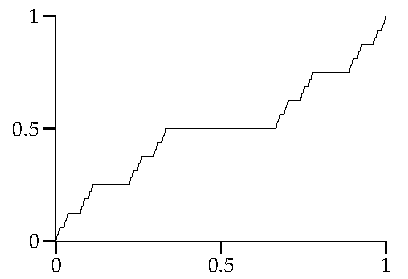
\includegraphics{figures/cantorfunction}
\caption{Cantor function or Devil's staircase (the function $\varphi$ from
the exercise).\label{fig:cantorfunction}}
\end{myfigureht}

\begin{exercise} \label{exercise:allowfiniteseqsinoutermeasure}
Prove that we obtain the same outer measure if we allow both finite and
infinite sequences in
the definition.  That is, define $\mu^*(S) \coloneqq \inf\, \sum_{j \in I} V(R_j)$
where the infimum is taken over all countable (finite or infinite) sets of
open rectangles $\{ R_j \}_{j\in I}$ such that $S \subset
\bigcup_{j \in I} R_j$.  Prove that for every $S \subset \R^n$,
$\mu^*(S) = m^*(S)$.
\end{exercise}

\begin{exercise}
Prove that for any two subsets $A, B \subset \R^n$, we have
$m^*(A \cup B) \leq m^*(A)+m^*(B)$.
\end{exercise}

\begin{exercise}
Suppose $A, B \subset \R^n$ are such that $m^*(B)=0$.  Prove that
$m^*(A \cup B) = m^*(A)$.
\end{exercise}

\begin{exercise}[Challenging] \label{exercise:outermeasureofsumofrectangles}
Suppose $R_1,R_2,\ldots,R_n$ are pairwise disjoint open rectangles.
Prove that 
$m^*(R_1 \cup R_2 \cup \cdots \cup R_n) = m^*(R_1)+m^*(R_2)+\cdots+m^*(R_n)$.
Hint: Some of the exercises above may prove very useful.
\end{exercise}


%%%%%%%%%%%%%%%%%%%%%%%%%%%%%%%%%%%%%%%%%%%%%%%%%%%%%%%%%%%%%%%%%%%%%%%%%%%%%%

\sectionnewpage
\section{The set of Riemann integrable functions }
\label{sec:riemannlebesgue}

\sectionnotes{1 lecture}

\subsection{Oscillation and continuity}

Consider
$D \subset \R^n$ and $f \colon D \to \R$.
Instead of just saying that $f$ is or is not continuous at
a point $x \in D$,
we want to quantify how discontinuous is $f$
at $x$.  For every $\delta > 0$, define the \emph{oscillation} of 
$f$ on the $\delta$-ball in subspace topology,
$B_D(x,\delta) = B_{\R^n}(x,\delta) \cap D$, as
\glsadd{not:oscillation}
\begin{equation*}
o(f,x,\delta) \coloneqq
{\sup_{y \in B_D(x,\delta)} f(y)}
-
{\inf_{y \in B_D(x,\delta)} f(y)}
= 
\sup_{y_1,y_2 \in B_D(x,\delta)} \bigl(f(y_1)-f(y_2)\bigr) .
\end{equation*}
That is, $o(f,x,\delta)$ is the length of the smallest interval
that contains the image $f\bigl(B_D(x,\delta)\bigr)$.
The definition makes sense for unbounded functions, where the oscillation
can be $\infty$, although we will mainly consider bounded functions.
Clearly $o(f,x,\delta) \geq 0$ and
$o(f,x,\delta) \leq o(f,x,\delta')$ whenever $\delta < \delta'$.
Therefore, the limit as $\delta \to 0$ from the right exists, and
we define the \emph{\myindex{oscillation}} of $f$
at $x$ as
\begin{equation*}
o(f,x) \coloneqq
\lim_{\delta \to 0^+}
o(f,x,\delta) =
\inf_{\delta > 0}
o(f,x,\delta) .
\end{equation*}

We will prove that function is continuous at $x$ if and only if $o(f,x) = 0$.
Fox example, if $f \colon \R \to \R$ is the Dirichlet function where
$f(x)=1$ if $x \in \Q$ and $f(x)=0$ otherwise, then $o(f,x) = 1$ for every
$x$, as any interval contains both rational and irrational numbers.
Accordingly, $f$ is not continuous at any $x$.
For another example, which is perhaps the origin of the terminology,
let $g \colon \R \to \R$ be given by
$g(x) = \sin(\nicefrac{1}{x})$ for $x\neq 0$ and $g(0)=0$,
see \figureref{fig:sin1xosc}.
Then at the discontinuity at $x=0$, we find $o(g,0) = 2$, as
in any neighborhood of $0$, the function takes both values $1$ and $-1$.
For all $x \neq 0$, the function is continuous and so, as we will see,
$o(g,x) = 0$.

\begin{myfigureht}
% also used in 3.1
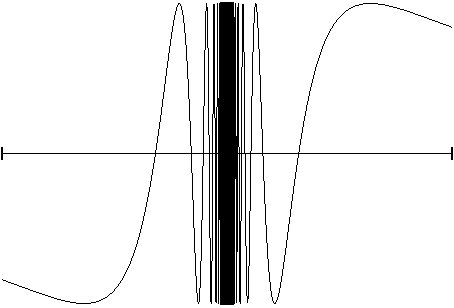
\includegraphics{figures/sin1xfig}
\caption{Graph of $\sin(\nicefrac{1}{x})$.\label{fig:sin1xosc}}
\end{myfigureht}

\begin{prop}
\pagebreak[2]
A function
$f \colon D \to \R$ is continuous at $x \in D$ if and only if $o(f,x) = 0$.
\end{prop}

\begin{proof}
First suppose that $f$ is continuous at $x \in D$.  Given $\epsilon > 0$,
there exists a $\delta > 0$ such that for $y \in B_D(x,\delta)$,
we have $\sabs{f(x)-f(y)} < \epsilon$.  Therefore, if $y_1,y_2 \in
B_D(x,\delta)$, then
\begin{equation*}
f(y_1)-f(y_2) =
\bigl(f(y_1)-f(x)\bigr)-\bigl(f(y_2)-f(x)\bigr) < \epsilon + \epsilon = 2 \epsilon .
\end{equation*}
Take the supremum over $y_1$ and $y_2$ to find
\begin{equation*}
o(f,x,\delta) = 
\sup_{y_1,y_2 \in B_D(x,\delta)} \bigl(f(y_1)-f(y_2)\bigr)
\leq
2 \epsilon .
\end{equation*}
As $o(x,f) \leq o(f,x,\delta) \leq 2\epsilon$, and $\epsilon > 0$ was arbitrary,
$o(x,f) = 0$.

On the other hand, suppose $o(x,f) = 0$.  Given $\epsilon > 0$,
find a $\delta > 0$ such that $o(f,x,\delta) < \epsilon$.  If
$y \in B_D(x,\delta)$, then
\begin{equation*}
\sabs{f(x)-f(y)}
\leq
\sup_{y_1,y_2 \in B_D(x,\delta)} \bigl(f(y_1)-f(y_2)\bigr)
=
o(f,x,\delta) < \epsilon. \qedhere
\end{equation*}
\end{proof}

\begin{prop} \label{prop:seclosed}
Let $D \subset \R^n$ be closed,
$f \colon D \to \R$, and $\epsilon > 0$.
The set $\bigl\{ x \in D : o(f,x) \geq \epsilon \bigr\}$ is closed.
\end{prop}

\begin{proof}
Equivalently, we want to show that
$G \coloneqq \bigl\{ x \in D : o(f,x) < \epsilon \bigr\}$ is open in the subspace topology.
Consider $x \in G$.
As $\inf_{\delta > 0} o(f,x,\delta) < \epsilon$, find a $\delta > 0$ such
that
\begin{equation*}
o(f,x,\delta) < \epsilon .
\end{equation*}
Take any $\xi \in B_D(x,\nicefrac{\delta}{2})$.  Notice that
$B_D(\xi,\nicefrac{\delta}{2}) \subset B_D(x,\delta)$.  Therefore,
\begin{equation*}
o(f,\xi,\nicefrac{\delta}{2}) =
\sup_{y_1,y_2 \in B_D(\xi,\nicefrac{\delta}{2})} \bigl(f(y_1)-f(y_2)\bigr) 
\leq
\sup_{y_1,y_2 \in B_D(x,\delta)} \bigl(f(y_1)-f(y_2)\bigr) = o(f,x,\delta) <
\epsilon .
\end{equation*}
So $o(f,\xi) < \epsilon$ as well.  As this is true for all $\xi \in
B_D(x,\nicefrac{\delta}{2})$, we get that $G$ is open in the subspace
topology, and $D \setminus G$ is closed as claimed.
\end{proof}


\subsection{The set of Riemann integrable functions}

We have seen that continuous functions are Riemann integrable, but we also
know that certain kinds of discontinuities are allowed.
It turns out that as long as the discontinuities happen on a set of measure
zero, the function is integrable, and vice versa.

\begin{thm}[Riemann--Lebesgue]\index{Riemann--Lebesgue theorem}
Let $R \subset \R^n$ be a closed rectangle and $f \colon R \to \R$
bounded.  Then $f$ is Riemann integrable if and only if
the set of discontinuities of $f$ is of measure zero.
\end{thm}

\begin{proof}
Let $S \subset R$ be the set of discontinuities of $f$, that is,
$S = \bigl\{ x \in R : o(f,x) > 0 \bigr\}$.
Suppose $S$ is a measure zero set: $m^*(S) = 0$.
The trick to proving that $f$ is integrable is to isolate the bad set
into a small set of subrectangles of a partition.  A partition has
finitely many subrectangles, so we need
compactness.  If $S$ were closed, then it would be compact and we could cover
it by finitely many small rectangles.  Unfortunately, $S$
itself is not closed in general, but the following set is.
Given $\epsilon > 0$, define
\begin{equation*}
S_\epsilon \coloneqq \bigl\{ x \in R : o(f,x) \geq \epsilon \bigr\} .
\end{equation*}
By \propref{prop:seclosed}, $S_\epsilon$ is closed,
and as it is also a subset of the bounded $R$,
$S_\epsilon$ is compact.  Moreover,
$S_\epsilon \subset S$ and $S$ is of measure zero,
so $S_\epsilon$ is of measure zero.
Via \propref{mv:prop:compactnull}, finitely many open rectangles
$O_1,O_2,\ldots,O_k$ cover $S_\epsilon$ and
$\sum_{j=1}^\infty V(O_j) < \epsilon$.  

The set $T \coloneqq R \setminus ( O_1 \cup \cdots \cup O_k )$ is closed, bounded,
and so compact.  As $o(f,x) < \epsilon$ for all $x \in T$,
for each $x \in T$, there is a $\delta > 0$ such that
$o(f,x,\delta) < \epsilon$, so there exists a small closed rectangle
$T_x \subset B(x,\delta)$ with $x$ in the interior of $T_x$, such that
\begin{equation*}
\sup_{y\in T_x} f(y) - \inf_{y\in T_x} f(y) < \epsilon.
\end{equation*}
The interiors of the rectangles $T_x$ cover $T$.  As $T$ is compact,
finitely many such rectangles $T_1, T_2, \ldots, T_m$
cover $T$.
Construct a partition $P$ out of the
endpoints of the rectangles $T_1,T_2,\ldots,T_m$
and $O_1,O_2,\ldots,O_k$ (ignoring those that
are outside the endpoints of $R$).  The
subrectangles $R_1,R_2,\ldots,R_p$ of $P$ are
such that every $R_j$ is contained in $T_\ell$ for some~$\ell$
or the closure of $O_\ell$ for some~$\ell$.  Order
the rectangles so that $R_1,R_2,\ldots,R_q$ are those
that are contained in some $T_\ell$, and $R_{q+1},R_{q+2},\ldots,R_{p}$
are the rest.
See \figureref{fig:nullsetintegrate}.
So
\begin{equation*}
\sum_{j=1}^q V(R_j) \leq V(R)
\qquad \text{and} \qquad
\sum_{j=q+1}^p V(R_j)
\leq
\sum_{\ell=1}^k V(O_\ell)
< \epsilon .
\end{equation*}
The second estimate holds because the $R_j$ that are subsets of $\widebar{O}_\ell$
give a partition of $\widebar{O}_\ell$ and hence their volumes sum to
$V(O_\ell)$.
Let $m_j$ and $M_j$ be the inf and sup of $f$ over $R_j$ as usual.
If $R_j \subset T_\ell$ for some $\ell$, then $M_j-m_j < \epsilon$.
Let $B \in \R$ be such that
$\sabs{f(x)} \leq B$ for all $x \in R$, so $M_j-m_j \leq 2B$ over all
rectangles. Then
\begin{equation*}
\begin{split}
U(P,f)-L(P,f)
& =
\sum_{j=1}^p (M_j-m_j) V(R_j)
\\
& =
\left(
\sum_{j=1}^q (M_j-m_j) V(R_j)
\right)
+
\left(
\sum_{j=q+1}^p (M_j-m_j) V(R_j)
\right)
\\
& <
\left(
\sum_{j=1}^q \epsilon\, V(R_j)
\right)
+
\left(
\sum_{j=q+1}^p 2 B\, V(R_j)
\right)
\\
& <
\epsilon\, V(R)
+
2B \epsilon = \epsilon \bigl(V(R)+2B\bigr) .
\end{split}
\avoidbreak
\end{equation*}
We can make the right-hand side as small as we want,
and hence $f$ is integrable.

\begin{myfigureht}
\subimport*{figures/}{nullsetintegrate.pdf_t}
\caption{A rectangle $R$ with $S_\epsilon$ marked as thick black line, and the
$O_\ell$ as shaded rectangles.  The partition is given by the dotted
lines.  Note how the $R_j$ partition the $O_\ell$.\label{fig:nullsetintegrate}}
\end{myfigureht}

\medskip

\pagebreak[2]
For the other direction, suppose $f$ is Riemann integrable
on $R$.
Let $S$ be the set of discontinuities of $f$ again.  Consider
the sequence of sets
\begin{equation*}
S_{1/k} = \bigl\{ x \in R : o(f,x) \geq \nicefrac{1}{k} \bigr\}.
\end{equation*}
Fix a $k \in \N$.
Given an $\epsilon > 0$, find a partition $P$ with subrectangles
$R_1,R_2,\ldots,R_p$ such that
\begin{equation*}
U(P,f)-L(P,f) =
\sum_{j=1}^p (M_j-m_j) V(R_j)
< \epsilon .
\end{equation*}
Suppose $R_1,R_2,\ldots,R_p$ are ordered so that
the interiors of $R_1,R_2,\ldots,R_{q}$ intersect $S_{1/k}$,
while the interiors of $R_{q+1},R_{q+2},\ldots,R_p$
are disjoint from $S_{1/k}$.
Let $R_j^\circ$ denote the interior of $R_j$.
Suppose $j \leq q$ and consider
$x \in R_j^\circ \cap S_{1/k}$.
Let $\delta > 0$ be small enough so that $B(x,\delta) \subset R_j$.
As $x \in S_{1/k}$, we get $o(f,x,\delta) \geq o(f,x) \geq \nicefrac{1}{k}$,
which, along with $B(x,\delta) \subset R_j$, implies
$M_j-m_j \geq \nicefrac{1}{k}$.
Then
\begin{equation*}
\epsilon >
\sum_{j=1}^p (M_j-m_j) V(R_j)
\geq
\sum_{j=1}^q (M_j-m_j) V(R_j)
\geq
\frac{1}{k}
\sum_{j=1}^q V(R_j) .
\end{equation*}
In other words,
$\sum_{j=1}^q V(R_j) < k \epsilon$.
Let $G$ be the set of all boundaries of all the subrectangles
of $P$.  The set $G$ is of measure zero (it can be covered by
finitely many sets from \exampleref{mv:example:planenull}).
We find
\begin{equation*}
S_{1/k} \subset R_1^\circ \cup R_2^\circ \cup \cdots \cup R_q^\circ \cup G .
\end{equation*}
As $G$ can also be covered by open rectangles arbitrarily small volume,
$S_{1/k}$ must be of measure zero.  As
\begin{equation*}
S = \bigcup_{k=1}^\infty S_{1/k}
\end{equation*}
and a countable union of measure zero sets is of measure zero, 
$S$ is of measure zero.
\end{proof}

\begin{cor} \label{cor:closednessofriemannintegrable}
\pagebreak[2]
Let $R \subset \R^n$ be a closed rectangle.  Let $\sR(R)$ be the set
of Riemann integrable functions on $R$.  Then
\begin{enumerate}[(i)]
\item
$\sR(R)$ is a real algebra:
If $f,g \in \sR(R)$ and $a \in \R$, then $af \in \sR(R)$, $f+g \in \sR(R)$
and $fg \in \sR(R)$.
\item
If $f,g \in \sR(R)$ and
\begin{equation*}
\varphi(x) \coloneqq \max \bigl\{ f(x) , g(x) \bigr\} ,
\qquad
\psi(x) \coloneqq \min \bigl\{ f(x) , g(x) \bigr\} ,
\end{equation*}
then $\varphi, \psi \in \sR(R)$.
\item
If $f \in \sR(R)$, then $\sabs{f} \in \sR(R)$, where $\sabs{f}(x) \coloneqq
\sabs{f(x)}$.
\item
If $R' \subset \R^n$ is another closed rectangle,
$U \subset \R^n$ and $U' \subset \R^n$ are open sets such that
$R \subset U$ and $R' \subset U'$,
$g \colon U \to U'$ is continuously differentiable, bijective,
$g^{-1}$ is continuously differentiable,
$g(R) \subset R'$,
and $f \in \sR(R')$,
then the composition $f \circ g$ is Riemann integrable on $R$.
\end{enumerate}
\end{cor}

The proof is contained in the exercises.

\subsection{Exercises}

\begin{exercise}
Suppose $f \colon (a,b) \times (c,d) \to \R$ is a bounded continuous
function.  Show that the integral of $f$ over $R = [a,b] \times [c,d]$ makes sense
and is uniquely defined.  That is, set $f$ to be anything (bounded) on the boundary of
$R$ and compute the integral, showing that the values on the boundary are
irrelevant.
\end{exercise}

\begin{exercise}
Suppose $R \subset \R^n$ is a closed rectangle.  Show that $\sR(R)$, the set
of Riemann integrable functions, is an algebra.  That is, show that
if $f,g \in \sR(R)$ and $a \in \R$, then $af \in \sR(R)$, $f+g \in \sR(R)$,
and $fg \in \sR(R)$.
\end{exercise}

\begin{exercise}
Suppose $R \subset \R^n$ is a closed rectangle and
$f \colon R \to \R$ is a bounded function which is zero except on a closed set $E
\subset R$ of measure
zero.  Show that $\int_R f$ exists and compute it.
\end{exercise}

\begin{exercise}
Suppose $R \subset \R^n$ is a closed rectangle and
$f \colon R \to \R$ and
$g \colon R \to \R$ are two Riemann integrable functions.  Suppose $f = g$
except for a closed set $E \subset R$ of measure zero.  Show that $\int_R f = \int_R g$.
\end{exercise}

\begin{samepage}
\begin{exercise}
Suppose $R \subset \R^n$ is a closed rectangle and
$f \colon R \to \R$ is a bounded function.
\begin{enumerate}[a)]
\item
Suppose there exists a closed set $E \subset R$ of measure zero such that
$f|_{R\setminus E}$ is continuous.  Then $f \in \sR(R)$.
\item
Find an example where $E \subset R$ is a set of measure zero
(not closed) such that
$f|_{R\setminus E}$ is continuous and $f \not\in \sR(R)$.
\end{enumerate}
\end{exercise}
\end{samepage}

\begin{exercise}
Suppose $R \subset \R^n$ is a closed rectangle
and $f \colon R \to \R$ and $g \colon R \to \R$ 
are Riemann integrable.
Show that
\begin{equation*}
\varphi(x) \coloneqq \max \bigl\{ f(x) , g(x) \bigr\} ,
\qquad
\psi(x) \coloneqq \min \bigl\{ f(x) , g(x) \bigr\} ,
\end{equation*}
are Riemann integrable.
\end{exercise}

\begin{exercise}
Suppose $R \subset \R^n$ is a closed rectangle
and $f \colon R \to \R$ is Riemann integrable.
Show that $\sabs{f}$ is Riemann integrable.
Hint: Define
$f_+(x) \coloneqq \max \bigl\{ f(x) , 0 \bigr\}$ and
$f_-(x) \coloneqq \max \bigl\{ -f(x) , 0 \bigr\}$, and then write $\sabs{f}$
in terms of $f_+$ and $f_-$.
\end{exercise}

\begin{exercise}
\leavevmode
\begin{enumerate}[a)]
\item
Suppose $R \subset \R^n$ and
$R' \subset \R^n$ are closed rectangles,
$U \subset \R^n$ and $U' \subset \R^n$ are open sets such that
$R \subset U$ and $R' \subset U'$,
$g \colon U \to U'$ is continuously differentiable, bijective,
$g^{-1}$ is continuously differentiable,
$g(R) \subset R'$, and
$f \in \sR(R')$, 
then the composition $f \circ g$ is Riemann integrable on $R$.
\item
Find a counterexample when $g$ is not one-to-one.
Hint: Try $g(x,y) \coloneqq (x,0)$ and $R=R'=[0,1] \times [0,1]$.
\end{enumerate}
\end{exercise}

\begin{exercise}
Suppose 
$f \colon [0,1]^2 \to \R$ is defined by
\begin{equation*}
f(x,y) \coloneqq
\begin{cases}
\frac{1}{kq} & \text{if } x,y \in \Q \text{ and } x = \frac{\ell}{k}
\text{ and } y=\frac{p}{q} \text{ in lowest terms,} \\
0            & \text{else.}
\end{cases}
\end{equation*}
Show that $f \in \sR\bigl({[0,1]}^2\bigr)$.
\end{exercise}

\begin{exercise}
Compute the oscillation $o\bigl(f,(x,y)\bigr)$ for all $(x,y) \in \R^2$
for the function
\begin{equation*}
f(x,y) \coloneqq
\begin{cases}
\frac{xy}{x^2+y^2} & \text{if } (x,y) \not= (0,0), \\
0                  & \text{if } (x,y) = (0,0) .
\end{cases}
\end{equation*}
\end{exercise}

\begin{exercise}
Consider the popcorn function $f \colon [0,1] \to \R$,
\begin{equation*}
f(x) \coloneqq
\begin{cases}
\frac{1}{q} & \text{if } x \in \Q \text{ and } x = \frac{p}{q}
 \text{ in lowest terms,} \\
0           & \text{else.}
\end{cases}
\end{equation*}
Compute $o(f,x)$ for all $x \in [0,1]$.
\end{exercise}

\begin{exercise}
Suppose $f \colon [a,b] \to \R$ and $g \colon [c,d] \to \R$ are Riemann integrable.
Show that $h \colon [a,b] \times [c,d] \to \R$ defined by $h(x,y) \coloneqq
f(x) g(y)$ is Riemann integrable and
\begin{equation*}
\int_{[a,b] \times [c,d]} h =
\left( \int_a^b f \right)
\left( \int_c^d g \right) .
\end{equation*}
\end{exercise}

\begin{exercise}
Let $R \subset \R^n$ be a closed rectangle and $f \colon R \to \R$ a
Riemann integrable function such that $f(x) \geq 0$ for all $x \in R$.
Show that if $\int_R f = 0$, then there is a measure zero set $E \subset R$ such that
$f(x) = 0$ for all $x \in R \setminus E$
(one says \myquote{$f=0$ \myindex{almost everywhere}}).
Note: This exercise in particular implies the rather subtle statement: If $f(x) > 0$
for all $x \in R$, then $\int_R f > 0$.
\end{exercise}


%%%%%%%%%%%%%%%%%%%%%%%%%%%%%%%%%%%%%%%%%%%%%%%%%%%%%%%%%%%%%%%%%%%%%%%%%%%%%%

\sectionnewpage
\section{Jordan measurable sets}
\label{sec:jordansets}

\sectionnotes{1--1.5 lecture}

\subsection{Volume and Jordan measurable sets}

Given a set
$S \subset \R^n$, its \emph{\myindex{characteristic function}}
or \emph{\myindex{indicator function}} $\chi_S \colon \R^n \to \R$
is defined by
\glsadd{not:indicatorfunction}
\begin{equation*}
\chi_S(x) \coloneqq
\begin{cases}
1 & \text{if } x \in S, \\
0 & \text{if } x \notin S.
\end{cases}
\end{equation*}
A bounded set $S$ is \emph{\myindex{Jordan measurable}}\footnote{Named after
the French mathematician
\href{https://en.wikipedia.org/wiki/Camille_Jordan}{Marie Ennemond Camille Jordan}
(1838--1922).}
if for some closed rectangle $R$ such that $S \subset R$, the function
$\chi_S$ is Riemann integrable, that is, $\chi_S \in \sR(R)$.
Take two closed rectangles $R$ and $R'$ 
with $S \subset R$ and $S \subset R'$, then $R \cap R'$ is a closed rectangle
also containing $S$.  By \propref{mv:prop:integralsmallerset}
and \exerciseref{mv:zerooutside}, $\chi_S \in \sR(R \cap R')$
and so $\chi_S \in \sR(R')$.  Thus
\begin{equation*}
\int_R \chi_S = \int_{R'} \chi_S = \int_{R \cap R'} \chi_S.
\end{equation*}
We define the
\emph{$n$-dimensional volume}%
\index{n-dimensional volume@$n$-dimensional volume!Jordan measurable set}%
\index{volume} of the
bounded Jordan measurable set $S$ as
\glsadd{not:ndimvolume}
\begin{equation*}
V(S) \coloneqq \int_R \chi_S ,
\end{equation*}
where $R$ is any closed rectangle containing $S$.

\begin{prop}
A bounded set $S \subset \R^n$ is Jordan measurable if and only if
the boundary $\partial S$ is a measure zero set.
\end{prop}

\begin{proof}
Suppose $R$ is a closed rectangle such that $S$ is
contained in the interior of $R$.
If $x \in \partial S$, then for every $\delta > 0$,
the sets $S \cap B(x,\delta)$ (where $\chi_S$ is 1) and
the sets $(R \setminus S) \cap B(x,\delta)$ (where $\chi_S$ is 0) are
both nonempty.  So $\chi_S$ is not continuous at $x$.
If $x$ is either in the interior of $S$ or in the complement of the closure
$\widebar{S}$, then $\chi_S$ is either identically 1 or identically 0
in a whole neighborhood of $x$ and hence $\chi_S$ is continuous at $x$.
Therefore, the set of discontinuities of $\chi_S$ is precisely the
boundary $\partial S$.  The proposition follows.
\end{proof}

\begin{prop} \label{prop:jordanmeas}
Suppose $S$ and $T$ are bounded Jordan measurable sets.
Then
\begin{enumerate}[(i)]
\item The closure $\widebar{S}$ is Jordan measurable.
\item The interior $S^\circ$ is Jordan measurable.
\item $S \cup T$ is Jordan measurable.
\item $S \cap T$ is Jordan measurable.
\item $S \setminus T$ is Jordan measurable.
\end{enumerate}
\end{prop}

The proof of the proposition is left as an exercise.
Next, we find that the volume that we defined above coincides with the outer
measure we defined above.

\begin{prop}
If $S \subset \R^n$ is Jordan measurable, then $V(S) = m^*(S)$.
\end{prop}

\begin{proof}
Given $\epsilon > 0$,
let $R$ be a closed rectangle that contains $S$.  Let $P$ be a partition
of $R$ such that 
\begin{equation*}
U(P,\chi_S) \leq \left( \int_R \chi_S \right) + \epsilon = V(S) + \epsilon
\qquad \text{and} \qquad
L(P,\chi_S) \geq \left( \int_R \chi_S \right) - \epsilon = V(S)-\epsilon.
\end{equation*}
Let $R_1,R_2,\ldots,R_k$ be all the subrectangles of $P$ such that $\chi_S$ is not
identically zero on each $R_j$.  That is, there is some point $x \in R_j$ such
that $x \in S$ (i.e.\ $\chi_S(x)=1$).  Let $O_j$ be an open rectangle such that $R_j \subset O_j$
and $V(O_j) < V(R_j) + \nicefrac{\epsilon}{k}$.  Notice that $S \subset
\bigcup_j O_j$.  Then
\begin{equation*}
U(P,\chi_S) = \sum_{j=1}^k V(R_j) > 
\left(\sum_{j=1}^k V(O_j)\right) - \epsilon \geq m^*(S) - \epsilon .
\end{equation*}
As 
$U(P,\chi_S) \leq V(S) + \epsilon$, then
$m^*(S) - \epsilon \leq V(S) + \epsilon$, or in other words
$m^*(S) \leq V(S)$.

Let $R'_1,R'_2,\ldots,R'_\ell$ be all the subrectangles of $P$ such that
$\chi_S$ is identically one on each $R'_j$.  In other words,
these are the subrectangles contained in $S$.
  The interiors
of the subrectangles $R'^\circ_j$ are disjoint and
$V(R'^\circ_j) = V(R'_j)$.  Via
\exerciseref{exercise:outermeasureofsumofrectangles},
\begin{equation*}
m^*\Bigl(\bigcup_{j=1}^\ell R'^\circ_j\Bigr)
=
\sum_{j=1}^\ell
V(R'^\circ_j) .
\end{equation*}
Hence
\begin{equation*}
m^*(S) \geq
m^*\Bigl(\bigcup_{j=1}^\ell R'_j\Bigr)
\geq
m^*\Bigl(\bigcup_{j=1}^\ell R'^\circ_j\Bigr)
=
\sum_{j=1}^\ell
V(R'^\circ_j)
=
\sum_{j=1}^\ell
V(R'_j)
=
L(P,f) \geq V(S) - \epsilon .
\end{equation*}
Therefore $m^*(S) \geq V(S)$ as well.
\end{proof}

\subsection{Integration over Jordan measurable sets}

In $\R$ there is only one reasonable type of set to integrate over:
an interval.   In $\R^n$ there are many kinds of sets.  The ones
that work with the Riemann integral are the Jordan measurable sets.

\begin{defn}
Let $S \subset \R^n$ be a bounded Jordan measurable set.
A bounded function $f \colon S \to \R$
is said to be
\emph{\myindex{Riemann integrable on $S$}}\index{integrable on $S$},
or\glsadd{not:integrablefuncR} $f \in \sR(S)$, if for a closed
rectangle $R$ such that $S \subset R$, the function $\widetilde{f} \colon R
\to \R$ defined by
\begin{equation*}
\widetilde{f}(x) \coloneqq
\begin{cases}
f(x) & \text{if } x \in S, \\
0 & \text{otherwise},
\end{cases}
\end{equation*}
is in $\sR(R)$.  In this case we write
\glsadd{not:riemannintR}%
\begin{equation*}
\int_S f \coloneqq \int_R \widetilde{f}.
\end{equation*}
\end{defn}

When $f$ is defined on a larger set and we wish to integrate over $S$, then
we apply the definition to the restriction $f|_S$.
As the restriction can be defined by the product $f\xi_S$, and the product
of Riemann integrable functions is Riemann integrable, $f|_S$ is automatically
Riemann integrable.
  In particular, 
if $f \colon R \to \R$ for a closed rectangle $R$, and $S \subset R$ is
a Jordan measurable subset, then
\begin{equation*}
\int_S f = \int_R f \chi_S .
\end{equation*}

\begin{prop}
If $S \subset \R^n$ is a bounded Jordan measurable set and $f \colon S \to \R$
is a bounded continuous function, then $f$ is integrable on $S$.
\end{prop}

\begin{proof}
Define the function $\widetilde{f}$ as above for some closed rectangle $R$ with $S
\subset R$.  If $x \in R \setminus \widebar{S}$, then $\widetilde{f}$
is identically zero in a neighborhood of $x$.  Similarly if $x$ is in the
interior of $S$, then $\widetilde{f} = f$ on a neighborhood of $x$
and $f$ is continuous at $x$.  Therefore, $\widetilde{f}$ is only ever
possibly discontinuous at $\partial S$, which is a set of measure zero,
and we are finished.
\end{proof}

We say some property
\emph{\myindex{for almost every} $x$}\index{almost every} if it holds
for all $x$ except on a set of measure zero.  We can also just say that
it happens \emph{\myindex{almost everywhere}}.
For example,
we say $f \colon S \to \R$ and $g \colon S \to \R$ are equal almost
everywhere if there exists a measure zero set $E \subset S$ such that
$f(x) = g(x)$ for all $x \in S \setminus E$.

\medskip

Many of the standard properties of the integral just carry over easily
since we are really integrating over a rectangle.  Furthermore, we can
make some of the statements to be \emph{almost everywhere}.
Proofs of the following three propositions left as exercises.

\begin{prop} \label{prop:jordanintbasic}
Suppose $S \subset \R^n$ is a bounded Jordan measurable set
and $f \colon S \to \R$ and
$g \colon S \to \R$ are Riemann integrable on $S$, and $\alpha \in \R$.
Then
\begin{enumerate}[(i)]
\item
If $f = 0$ almost everywhere, then $\int_S f = 0$.
\item
If $f = g$ almost everywhere, then $\int_S f = \int_S g$.
\item
$f+g$ is Riemann integrable on $S$ and $\int_S (f+g) = \int_S f + \int_S
g$.
\item
$\alpha f$ is Riemann integrable on $S$ and $\int_S \alpha f = \alpha \int_S f$.
\item
If $f(x) \leq g(x)$ for almost every $x$, then $\int_S f \leq \int_S g$.
\end{enumerate}
\end{prop}

We also have additivity.

\begin{prop} \label{prop:jordanintadd}
Suppose $A \subset \R^n$ and $B \subset \R^n$ are disjoint bounded Jordan
measurable sets and $f \colon A \cup B \to \R$
is such that the restrictions $f|_A$ and $f|_B$
are Riemann integrable on $A$ and $B$ respectively.
Then $f$ is Riemann integrable on $A \cup B$
and
\begin{equation*}
\int_{A \cup B} f = \int_A f + \int_B f .
\end{equation*}
\end{prop}

Finally, to integrate over non-rectangular regions using Fubini's theorem,
the typical way is to cut the region into simpler pieces that can be
described by two graphs.  We state the theorem in the plane, but similar
statements can be made in more variables.  The proof is again left as an
exercise.

\begin{prop} \label{prop:intovertypeIset}
Let $f \colon [a,b] \to \R$ and
$g \colon [a,b] \to \R$ be continuous functions and such that
for all $x \in (a,b)$, $f(x) < g(x)$.  Let
\begin{equation*}
U \coloneqq \bigl\{ (x,y) \in \R^2 : a < x < b \text{ and } f(x) < y < g(x) \bigr\} .
\end{equation*}
See \figureref{fig:typeIdomain}.
Then $U$ is Jordan measurable, and if 
$\varphi \colon U \to \R$ is Riemann integrable on $U$, then
\begin{equation*}
\int_U \varphi =
\int_a^b \int_{f(x)}^{g(x)} \varphi(x,y) \, dy \, dx .
\end{equation*}
\end{prop}

\begin{myfigureht}
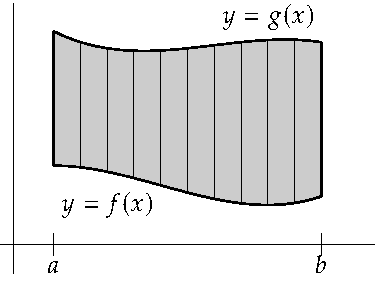
\includegraphics{figures/typeIdomain}
\caption{Domain between two graphs.\label{fig:typeIdomain}}
\end{myfigureht}

\subsection{Images of Jordan measurable subsets}

Finally, images of Jordan measurable sets are Jordan measurable under
nice enough mappings.  For simplicity, we assume that the Jacobian
determinant never vanishes.

\begin{prop} \label{prop:imagejordanmeas}
Suppose $U \subset \R^n$ is open and
$S \subset U$ is a compact Jordan measurable set.
Suppose
$g \colon U \to \R^n$ is a one-to-one
continuously differentiable mapping such that
the Jacobian determinant $J_g$ is never zero on $S$.
Then $g(S)$ is bounded and Jordan measurable.
\end{prop}

\begin{proof}
Let $T \coloneqq g(S)$.  %As $S \subset \R^n$ is closed and bounded it is compact.
By 
\volIref{\lemmaref*{vI-lemma:continuouscompact} from volume I}{\lemmaref{lemma:continuouscompact}},
the set
$T$ is also compact and so closed and bounded.
We claim $\partial T \subset g(\partial S)$.  Suppose the claim is proved.
As $S$ is Jordan measurable, then
$\partial S$ is measure zero.  Then  $g(\partial S)$ is measure
zero by \propref{prop:imagenull}.  As $\partial T \subset g(\partial
S)$, then $T$ is Jordan measurable.

It is therefore left to prove the claim.
As $T$ is closed, $\partial T \subset T$.
Suppose $y \in \partial T$, then there must exist an
$x \in S$
such that $g(x) = y$, and by hypothesis $J_g(x) \not= 0$.
We use the inverse function theorem (\thmref{thm:inverse}).  We find 
a neighborhood $V \subset U$ of $x$ and an open set $W$ such that
the restriction $f|_V$ is a one-to-one and onto function from $V$ to $W$
with a continuously differentiable inverse.  In particular, $g(x) = y \in W$.
As $y \in \partial T$, there exists a sequence $\{ y_k \}_{k=1}^\infty$ in $W$ with
$\lim_{k\to\infty} y_k = y$ and $y_k \notin T$.  As $g|_V$ is invertible and in
particular has a continuous inverse, there exists
a sequence $\{ x_k \}_{k=1}^\infty$ in $V$ such that $g(x_k) = y_k$ and
$\lim_{k\to\infty} x_k = x$.
Since $y_k \notin T = g(S)$, clearly $x_k \notin S$.  Since $x \in S$, we
conclude that $x \in \partial S$.  The claim is proved, $\partial T \subset
g(\partial S)$.
\end{proof}

\subsection{Exercises}

\begin{exercise}
Prove \propref{prop:jordanmeas}.
\end{exercise}

\begin{exercise}
Prove that a bounded convex set is Jordan measurable.  Hint: Induction on
dimension.
\end{exercise}

\begin{exercise} \label{exercise:intovertypeIset}
Prove \propref{prop:intovertypeIset}.  That is,
\begin{enumerate}[a)]
\item
Show that $U$ is Jordan measurable.
\item
Prove that
$\int_U \varphi =
\int_a^b \int_{f(x)}^{g(x)} \varphi(x,y) \, dy \, dx$.
\end{enumerate}
\end{exercise}

\begin{exercise}
Let us construct an example of a non-Jordan measurable open set.
Start in one dimension.  Let $\{ r_j \}_{j=1}^\infty$ be an enumeration
of all rational numbers in $(0,1)$.  Let $(a_j,b_j)$ be open intervals
such that $(a_j,b_j) \subset (0,1)$ for all $j$, $r_j \in (a_j,b_j)$,
and $\sum_{j=1}^\infty (b_j-a_j) < \nicefrac{1}{2}$.  Now let $U \coloneqq
\bigcup_{j=1}^\infty (a_j,b_j)$.
\begin{enumerate}[a)]
\item
Show the open intervals $(a_j,b_j)$ as above actually exist.
\item
Prove $\partial U = [0,1] \setminus U$.
\item
Prove $\partial U$ is not of measure zero, and therefore $U$ is not Jordan measurable.
\item
Show that $W \coloneqq
\bigl( U \times (0,2) \bigr) \cup \bigl( (0,1) \times (1,2) \bigr)$
is a connected bounded open set in $\R^2$
that is not Jordan measurable.
\end{enumerate}
\end{exercise}

\begin{exercise}
Suppose $K \subset \R^n$ is a closed measure zero set.
\begin{enumerate}[a)]
\item
If $K$ is bounded, prove that $K$ is Jordan measurable.
\item
If $S \subset \R^n$ is bounded and Jordan measurable, prove that
$S \setminus K$ is Jordan measurable.
\item
Construct a bounded Jordan measurable $S \subset \R^n$
and a bounded $T \subset \R^n$ of measure zero, such that
neither $T$ nor $S \setminus T$ is Jordan measurable.
\end{enumerate}
\end{exercise}

\begin{exercise}
Suppose $U \subset \R^n$ is open and $K \subset U$ is compact.
Find a compact Jordan measurable set $S$ such that $S \subset U$
and $K \subset S^\circ$ ($K$ is in the interior of $S$).
\end{exercise}

\begin{exercise} \label{exercise:closednessofriemannintegrable}
Prove a version of \corref{cor:closednessofriemannintegrable}, replacing all closed
rectangles with closed and bounded Jordan measurable sets.
\end{exercise}

\begin{exercise}
Prove \propref{prop:jordanintbasic}.
\end{exercise}

\begin{exercise}
Prove \propref{prop:jordanintadd}.
\end{exercise}

%%%%%%%%%%%%%%%%%%%%%%%%%%%%%%%%%%%%%%%%%%%%%%%%%%%%%%%%%%%%%%%%%%%%%%%%%%%%%%

\sectionnewpage
\section{Green's theorem}
\label{sec:mvgreenstheorem}

\sectionnotes{1 lecture, requires \chapterref{path:chapter}}

One of the most important theorems in the calculus of several variables is the
so-called generalized Stokes' theorem, a generalization of the
fundamental theorem of calculus.  The two-dimensional
version is called Green's theorem%
\footnote{Named after the British mathematical physicist
\href{https://en.wikipedia.org/wiki/George_Green_(mathematician)}{George Green}
(1793--1841).}.  We will state the theorem in general, but
we will only prove a special, but important, case.

\begin{defn}
Let $U \subset \R^2$ be a bounded connected open set.
Suppose the boundary
$\partial U$ is a disjoint union of (the images of) finitely many
simple closed piecewise smooth paths such that
every $p \in \partial U$ is in the closure of
$\R^2 \setminus \widebar{U}$.
Then $U$ is called a
\emph{\myindex{bounded domain with piecewise smooth boundary}}%
\index{piecewise smooth boundary}
in $\R^2$.
\end{defn}

The condition about points outside the closure says that locally $\partial U$
separates $\R^2$ into an \myquote{inside} and an \myquote{outside.}  The condition prevents
$\partial U$ from being just a \myquote{cut} inside $U$.  As we travel
along the path in a certain orientation,
there is a well-defined left and a right, and either $U$ is on the left
and the complement of $U$ is on the right, or vice versa.   
The orientation on $U$ is the direction in which we travel along the
paths.  We can switch orientation if needed by reparametrizing the
path.

\begin{defn}
Let $U \subset \R^2$ be a bounded domain with piecewise smooth boundary,
let $\partial U$ be oriented ,
and let $\gamma \colon [a,b] \to \R^2$ be a parametrization of $\partial U$
giving the orientation.  Write $\gamma(t) = \big(x(t),y(t)\bigr)$.
If the vector $n(t) \coloneqq \bigl(-y'(t),x'(t)\bigr)$ points into the domain,
that is, $\epsilon n(t) + \gamma(t)$ is in $U$ for all small enough
$\epsilon > 0$, then $\partial U$ is
\emph{\myindex{positively oriented}}.  
See \figureref{fig:positiveorient}.
Otherwise it is \emph{\myindex{negatively oriented}}.
\end{defn}

\begin{myfigureht}
\subimport*{figures/}{positiveorient.pdf_t}
\caption{Positively oriented domain (left), and a positively oriented
domain with a hole (right).\label{fig:positiveorient}}
\end{myfigureht}

The vector $n(t)$ turns $\gamma^{\:\prime}(t)$
counterclockwise by $90^\circ$, that is to the left.
When we travel along a positively oriented boundary
in the direction of its orientation,
the domain is \myquote{on our left.}
For example,
if $U$ is a bounded domain with \myquote{no holes,} that is $\partial U$
is connected, then the positive orientation means we are traveling
counterclockwise around $\partial U$.  If we do have \myquote{holes,} then we
travel around them clockwise.

\begin{prop}
Let $U \subset \R^2$ be a bounded domain with piecewise smooth boundary.
Then $U$ is Jordan measurable.
\end{prop}

\begin{proof}
We must show that
$\partial U$ is a null set.  As $\partial U$ is a finite
union of piecewise smooth paths, which 
are finite unions of smooth paths, we need only show that 
a smooth path in $\R^2$ is a null set.
Let $\gamma \colon [a,b] \to \R^2$ be a smooth path.
It is enough to show that
$\gamma\bigl((a,b)\bigr)$ is a null set, as adding 
the points $\gamma(a)$ and $\gamma(b)$,
to a null set still results in a null set.
Define
\begin{equation*}
f \colon (a,b) \times (-1,1) \to \R^2,
\qquad \text{as} \qquad
f(x,y) \coloneqq \gamma(x) .
\end{equation*}
The set $(a,b) \times \{ 0 \}$ is a null set in $\R^2$ and
$\gamma\bigl((a,b)\bigr) = f\bigl( (a,b) \times \{ 0 \} \bigr)$.
By \propref{prop:imagenull}, 
$\gamma\bigl((a,b)\bigr)$ is a null set in $\R^2$
and so
$\gamma\bigl([a,b]\bigr)$ is a null set, and 
so finally $\partial U$ is a null set.
\end{proof}

\begin{thm}[Green]\index{Green's theorem}
Suppose $U \subset \R^2$ is a bounded domain with piecewise smooth boundary with
the boundary positively oriented.  Suppose $P$ and $Q$ are continuously
differentiable functions defined on some open set that contains the closure
$\widebar{U}$.  Then
\begin{equation*}
\int_{\partial U}
P \, dx + Q\,  dy
=
\int_{U}
\left(\frac{\partial Q}{\partial x} - \frac{\partial P}{\partial y} \right)
.
\end{equation*}
\end{thm}

We stated Green's theorem in general, although we will only prove a special 
version of it.  That is, we will only prove it for a special kind of domain.
The general version follows from the special case 
by application of further geometry, and cutting up the general
domain into smaller domains on which to apply the special case.
We will not prove the general case. 

Let $U \subset \R^2$ be a domain with piecewise smooth boundary.
We say $U$ is of \emph{type I}\index{type I domain}
if there exist numbers
$a < b$, and continuous
functions $f \colon [a,b] \to \R$ and
$g \colon [a,b] \to \R$, such that
\begin{equation*}
U \coloneqq \bigl\{ (x,y) \in \R^2 : a < x < b \text{ and } f(x) < y < g(x) \bigr\} .
\end{equation*}
Similarly, $U$ is of \emph{type II}\index{type II domain}
if there exist numbers
$c < d$, and continuous
functions $h \colon [c,d] \to \R$ and
$k \colon [c,d] \to \R$, such that
\begin{equation*}
U \coloneqq \bigl\{ (x,y) \in \R^2 : c < y < d \text{ and } h(y) < x < k(y) \bigr\} .
\end{equation*}
Finally, $U \subset \R^2$ is of \emph{type III}\index{type III domain}
if it is both of type I and type II\@.  See \figureref{fig:greenstypes}.

\begin{myfigureht}
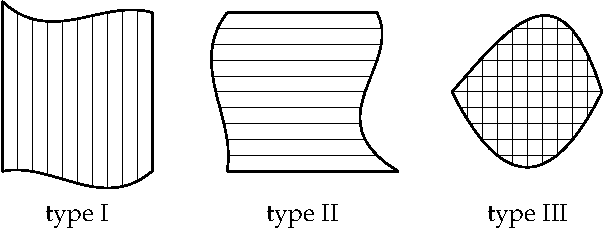
\includegraphics{figures/greenstypes}
\caption{Domain types for Green's theorem.\label{fig:greenstypes}}
\end{myfigureht}

Common domains to apply Green's theorem to are rectangles and discs, and
these are type III domains.
We will only prove Green's theorem for type III domains.

\begin{proof}[Proof of Green's theorem for $U$ of type III]
Let $f,g,h,k$ be the functions defined above.
Using \propref{prop:intovertypeIset},
$U$ is Jordan measurable and as $U$ is of type I\@, then
\begin{equation*}
\begin{split}
\int_U 
\left(- \frac{\partial P}{\partial y} \right)
& =
\int_a^b \int_{g(x)}^{f(x)}
\left(- \frac{\partial P}{\partial y} (x,y) \right)
\, dy \, dx 
\\
& =
\int_a^b \Bigl(
- P\bigl(x,f(x)\bigr) +
P\bigl(x,g(x)\bigr)
\Bigr) \, dx
\\
& =
\int_a^b P\bigl(x,g(x)\bigr) \, dx 
-
\int_a^b P\bigl(x,f(x)\bigr) \, dx .
\end{split}
\end{equation*}
We integrate $P\,dx$ along the boundary.
The one-form $P\,dx$ integrates to zero 
along the straight vertical lines in the boundary.  Therefore it is
only
integrated along the top and along the bottom.  As a parameter,
$x$ runs from left to right.  If we use the parametrizations that take $x$
to $\bigl(x,f(x)\bigr)$ and to
$\bigl(x,g(x)\bigr)$ we recognize path integrals above.  However the second
path integral is in the wrong direction; the top should be going right to
left, and so we must switch orientation.
\begin{equation*}
\int_{\partial U} P \, dx
=
\int_a^b P\bigl(x,g(x)\bigr) \, dx 
+
\int_b^a P\bigl(x,f(x)\bigr) \, dx
=
\int_U 
\left(- \frac{\partial P}{\partial y} \right) .
\end{equation*}

Similarly, $U$ is also of type II\@.  The form $Q\,dy$ integrates to zero along
horizontal lines.   So
\begin{equation*}
\int_U 
\frac{\partial Q}{\partial x}
=
\int_c^d \int_{k(y)}^{h(y)}
\frac{\partial Q}{\partial x}(x,y)
\, dx \, dy 
=
\int_a^b \Bigl(
Q\bigl(y,h(y)\bigr) 
-
Q\bigl(y,k(y)\bigr)
\Bigr) \, dx 
=
\int_{\partial U} Q \, dy .
\end{equation*}
Putting the two computations together we obtain
\begin{equation*}
\int_{\partial U} P\, dx + Q \, dy 
=
\int_{\partial U} P\, dx + \int_{\partial U} Q \, dy 
=
\int_U 
\Bigl(-\frac{\partial P}{\partial y}\Bigr)
+
\int_U 
\frac{\partial Q}{\partial x}
=
\int_U 
\Bigl(
\frac{\partial Q}{\partial x}
-\frac{\partial P}{\partial y}
\Bigr) . \qedhere
\end{equation*}
\end{proof}

Let's see how one can use the simple version of Green's for a more complex
path.

\begin{example}
Suppose $P(x,y) = \frac{-y}{x^2+y^2}$, 
$Q(x,y) = \frac{x}{x^2+y^2}$.  If we think of $(P,Q)$ as a vector, so that
we have a so-called \emph{\myindex{vector field}}, $(P,Q)$ is
called the \emph{\myindex{vortex vector field}}, as it gives the velocity
of particles traveling in a vortex around the origin.  Variations on this
vector field come up often in applications.
Suppose that $\gamma$ is a path that goes counterclockwise around
a rectangle whose interior contains the origin.
We claim
\begin{equation*}
\int_{\gamma} \frac{-y}{x^2+y^2} \, dx + \frac{x}{x^2+y^2} \, dy = 2 \pi .
\end{equation*}

First we draw a circle $C$ of radius $r > 0$ centered at the origin such
that the entire circle is within $\gamma$ and oriented clockwise.
Consider $U$ to be the domain between $\gamma$ and $C$.
See \figureref{fig:vortexbox}.
The integral around $\partial U$ is the integral around $\gamma$ plus the
integral around $C$.
Now $U$ is not a domain of type III so we cannot just apply the version of
Green's theorem we actually proved.
However, if we cut the box along the axis as shown in the figure with
dashed lines, the four resulting domains,
let us call them $U_1,U_2,U_3,U_4$,
are of type III.
The dashed lines are oriented in opposite directions
for the two $U_j$ that share them,
and so when we integrate along both,
 the integrals cancel.  That is,
\begin{multline*}
\int_{\partial U} P\, dx + Q \, dy
=
\\
\int_{\partial U_1} P\, dx + Q \, dy
+
\int_{\partial U_2} P\, dx + Q \, dy
+
\int_{\partial U_3} P\, dx + Q \, dy
+
\int_{\partial U_4} P\, dx + Q \, dy .
\end{multline*}
Now we can apply Green's theorem to every $U_j$.
We leave it to the reader to verify that outside of the origin,
$\frac{\partial Q}{\partial x} - \frac{\partial P}{\partial y} = 0$.
So 
\begin{equation*}
\int_{\partial U_j} P\, dx + Q \, dy 
=
\int_{U_j} \left( \frac{\partial Q}{\partial x} - \frac{\partial P}{\partial
y} \right)
=
\int_{U_j} 0 = 0 .
\end{equation*}
Next we notice that
\begin{equation*}
\int_C P \, dx + Q \, dy
+
\int_{\gamma} P \, dx + Q \, dy
=
\int_{\partial U} P \, dx + Q \, dy = 0 .
\end{equation*}
So the integral around $C$ is minus the integral around $\gamma$.  The
integral around $C$ is easy to compute as on $C$ we have $x^2+y^2 = r^2$,
so $P(x,y) = \frac{-y}{r^2}$ and $Q(x,y) = \frac{x}{r^2}$.
We leave it to the reader to compute
\begin{equation*}
\int_C P\, dx + Q \, dy
=
\int_C \frac{-y}{r^2}\, dx + \frac{x}{r^2} \, dy
=
- 2 \pi .
\end{equation*}
The claim follows.
\begin{myfigureht}
\subimport*{figures/}{vortexbox.pdf_t}
\caption{Changing the box integral to an integral around a small circle around
the origin.  The domain $U$ is the shaded area between the circle and the
box.\label{fig:vortexbox}}
\end{myfigureht}

We remark that if $\gamma$ would not contain the origin, $\int_\gamma
P\,dx+Q\,dy = 0$, as we could just apply Green's to $\gamma$.
So this integral can detect whether the origin is inside $\gamma$ or not.
\end{example}

As a second example, we illustrate the usefulness of Green's theorem on a fundamental result
about harmonic functions.

\begin{example}
Suppose $U \subset \R^2$ is open and
$f \colon U \to \R$ is harmonic, that is, $f$ is twice continuously
differentiable and
satisfies the \emph{\myindex{Laplace equation}},
$\frac{\partial^2 f}{\partial x^2} +
\frac{\partial^2 f}{\partial y^2} = 0$.
Harmonic functions are, for instance, the steady state heat distribution,
or the electric potential between charges.
We will prove one of the most fundamental properties of these functions.

Let $D_r \coloneqq B(p,r)$ be a disc such that its closure $C(p,r) \subset U$.  Write
$p = (x_0,y_0)$.  We orient
$\partial D_r$ positively.  See \exerciseref{green:balltype3orient}.
Then
\begin{equation*}
\begin{split}
0
& =
\frac{1}{2\pi r}
\int_{D_r}
\left(
\frac{\partial^2 f}{\partial x^2} +
\frac{\partial^2 f}{\partial y^2}
\right)
\\
& 
=
\frac{1}{2\pi r}
\int_{\partial D_r}
- \frac{\partial f}{\partial y} \, dx + 
\frac{\partial f}{\partial x} \, dy
\\
&
=
\frac{1}{2\pi r}
\int_0^{2\pi}
\biggl(
- \frac{\partial f}{\partial y} \bigl(x_0+r\cos(t),y_0+r\sin(t)\bigr) \bigl(-r\sin(t)\bigr)
\\
& \hspace{1.2in}
+ \frac{\partial f}{\partial x} \bigl(x_0+r\cos(t),y_0+r\sin(t)\bigr) r\cos(t)
\biggr) \, dt
\\
&
=
\frac{d}{dr}
\left[
\frac{1}{2\pi}
\int_0^{2\pi}
f\bigl(x_0+r\cos(t),y_0+r\sin(t)\bigr) \, dt
\right] .
\end{split}
\end{equation*}
Let $g(r) \coloneqq 
\frac{1}{2\pi}
\int_0^{2\pi}
f\bigl(x_0+r\cos(t),y_0+r\sin(t)\bigr) \, dt$.  Then $g'(r) = 0$ for all
$r > 0$.
The function is constant for $r >0$ and continuous at $r=0$ (exercise).
Therefore, $g(0) = g(r)$ for all $r > 0$, and
\begin{equation*}
g(r) = g(0) = 
\frac{1}{2\pi}
\int_0^{2\pi}
f\bigl(x_0+0\cos(t),y_0+0\sin(t)\bigr) \, dt
=
f(x_0,y_0).
\end{equation*}
We
proved the \emph{\myindex{mean value property}} of harmonic functions:
\begin{equation*}
f(x_0,y_0) = 
\frac{1}{2\pi}
\int_0^{2\pi}
f\bigl(x_0+r\cos(t),y_0+r\sin(t)\bigr) \, dt 
=
\frac{1}{2\pi r}
\int_{\partial D_r} f \, ds .
\end{equation*}
That is, for a harmonic function, the value at $p = (x_0,y_0)$ is the average
over a circle of any radius $r$ centered at $(x_0,y_0)$.
\end{example}

\subsection{Exercises}

\begin{exercise} \label{green:balltype3orient}
Prove that a disc $B(p,r) \subset \R^2$ is a type III domain, and prove that
the orientation given by the parametrization $\gamma(t) =
\bigl(x_0+r\cos(t),y_0+r\sin(t)\bigr)$ where $p = (x_0,y_0)$ is the positive
orientation of the boundary $\partial B(p,r)$.
\\
Note: Feel free to use what you know about sine and cosine from calculus.
\end{exercise}

\begin{exercise}
Prove that a convex bounded domain with piecewise smooth boundary
is a type III domain.
\end{exercise}

\begin{exercise}
Suppose $V \subset \R^2$ is a domain with piecewise smooth boundary that is
a type III domain and suppose that $U \subset \R^2$ is a domain such that
$\widebar{V} \subset U$.  Suppose $f \colon U \to \R$ is a twice
continuously differentiable function.  Prove that
$\int_{\partial V}
\frac{\partial f}{\partial x} \, dx + 
\frac{\partial f}{\partial y} \, dy = 0$.
\end{exercise}

\begin{samepage}
\begin{exercise}
For a disc $B(p,r) \subset \R^2$, orient the boundary $\partial B(p,r)$
positively.
\begin{enumerate}[a)]
\item
Compute $\displaystyle \int_{\partial B(p,r)} -y \, dx$.
\item
Compute $\displaystyle \int_{\partial B(p,r)} x \, dy$.
\item
Compute $\displaystyle \int_{\partial B(p,r)} \frac{-y}{2} \, dx +
\frac{x}{2} \, dy$.
\end{enumerate}
\end{exercise}
\end{samepage}

\begin{exercise}
Using Green's theorem show that the area of a triangle with
vertices
$(x_1,y_1)$,
$(x_2,y_2)$,
$(x_3,y_3)$ is
$\frac{1}{2}\sabs{x_1y_2 + x_2 y_3 + x_3 y_1 - y_1x_2 - y_2x_3 - y_3x_1}$.
Hint: See previous exercise.
\end{exercise}

\begin{exercise}
Using the mean value property prove the
\emph{maximum principle}\index{maximum principle!harmonic functions}
for harmonic functions:
Suppose $U \subset \R^2$ is a connected open set and
$f \colon U \to \R$ is harmonic. Prove that
if $f$ attains a maximum at $p \in U$, then $f$ is constant.
\end{exercise}

\begin{exercise}
Let $f(x,y) \coloneqq \ln \sqrt{x^2+y^2}$.
\begin{enumerate}[a)]
\item
Show $f$ is harmonic where defined.
\item
Show $\lim\limits_{(x,y) \to 0} f(x,y) = -\infty$.
\item
Using a circle $C_r$ of radius
$r$ around the origin, compute $\frac{1}{2\pi r} \int_{\partial C_r} f \, ds$.
What happens as $r \to 0$?
\item
Why can't you use Green's theorem?
\end{enumerate}
\end{exercise}


%%%%%%%%%%%%%%%%%%%%%%%%%%%%%%%%%%%%%%%%%%%%%%%%%%%%%%%%%%%%%%%%%%%%%%%%%%%%%%

\sectionnewpage
\section{Change of variables}
\label{sec:mvchangeofvars}

\sectionnotes{1 lecture}

In one variable, we have the familiar change of variables
\begin{equation*}
\int_a^b f\bigl(g(x)\bigr) g'(x)\, dx = 
\int_{g(a)}^{g(b)} f(x) \, dx .
\end{equation*}
The analogue in higher dimensions is quite
a bit more complicated.  The first complication is orientation.  If we use
the definition of integral from this chapter, then we do not have the notion
of $\int_a^b$ versus $\int_b^a$.  We are simply integrating over an
interval $[a,b]$.  With this notation, the change of variables becomes
\begin{equation*}
\int_{[a,b]} f\bigl(g(x)\bigr) \, \sabs{g'(x)}\, dx = 
\int_{g([a,b])} f(x) \, dx .
\end{equation*}
In this section we will obtain the several-variable analogue of this form.

Let us remark the role of $\sabs{g'(x)}$ in the formula. 
The integral measures volumes in general, so in one dimension it measures length.
Notice that $\sabs{g'(x)}$ scales the $dx$ and
so it scales the lengths.
If our $g$ is linear, that is, $g(x)=Lx$, then
$g'(x) = L$ and the length of the interval $g([a,b])$ is simply
$\sabs{L}(b-a)$.  That is because $g([a,b])$ is either $[La,Lb]$ or
$[Lb,La]$.  This property holds in higher dimension with $\sabs{L}$ replaced
by the absolute value of the determinant.

\begin{prop} \label{prop:volrectdet}
Suppose $R \subset \R^n$ is a rectangle
and $A \colon \R^n \to \R^n$ is linear.  Then
$A(R)$ is Jordan measurable and $V\bigl(A(R)\bigr) = \sabs{\det (A)} \, V(R)$.
\end{prop}

\begin{proof}
It is enough to prove for elementary matrices.  The proof is left as an
exercise.
\end{proof}

Let us prove that
absolute value of the Jacobian determinant
$\sabs{J_g(x)} = \babs{\det \bigl(g'(x)\bigr)}$
is the replacement of $\sabs{g'(x)}$ for multiple
dimensions in the change of variables formula.
The following theorem holds in more generality,
but this statement is sufficient for many uses.

\begin{thm}
Suppose $U \subset \R^n$ is open,
$S \subset U$ is a compact Jordan measurable set, and
$g \colon U \to \R^n$ is a one-to-one
continuously differentiable mapping, such that
$J_g$ is never zero on $S$.
Suppose $f \colon g(S) \to \R$ is Riemann integrable.
Then $f \circ g$ is Riemann integrable on $S$ and
\begin{equation*}
\int_{g(S)} f(x) \, dx = 
\int_S f\bigl(g(x)\bigr) \, \sabs{J_g(x)} \, dx .
\end{equation*}
\end{thm}

The set $g(S)$ is Jordan measurable by \propref{prop:imagejordanmeas},
so the left-hand side does make sense.
That the right-hand side makes sense follows by
\corref{cor:closednessofriemannintegrable} (actually
\exerciseref{exercise:closednessofriemannintegrable}).

\begin{proof}
The set $S$ can be covered by finitely many closed rectangles
$P_1,P_2,\ldots,P_k$, whose
interiors do not overlap such that each $P_j \subset U$
(\exerciseref{mv:changeofvarcoverbyrects}).
Proving the theorem for $P_j \cap S$ instead of $S$ is enough.
Define $f(y) \coloneqq 0$ for all $y \notin g(S)$.
The new $f$ is still Riemann integrable since $g(S)$ is Jordan measurable.
We can now replace the integrals over $S$ with integrals over the whole
rectangle.
We therefore assume that $S$ is equal to a rectangle $R$.

Let $\epsilon > 0$ be given.
For every $x \in R$, let
\begin{equation*}
W_x \coloneqq \bigl\{ y \in U : \snorm{g'(x)-g'(y)} < \nicefrac{\epsilon}{2} \bigr\} .
\end{equation*}
By \exerciseref{mv:changeofvarWxopen},
$W_x$ is open.
As $x \in W_x$ for every $x$, it is an open cover.
By the Lebesgue covering lemma
(\volIref{\lemmaref*{vI-ms:lebesgue} from volume I}{\lemmaref{ms:lebesgue}}),
there exists a $\delta > 0$ such that
for every $y \in R$, there is an $x$ such that $B(y,\delta) \subset W_x$.
In other words, if $P$ is a rectangle of maximum side length less
than $\frac{\delta}{\sqrt{n}}$ and $y \in P$, then $P \subset
B(y,\delta) \subset W_x$.  By triangle inequality,
$\snorm{g'(\xi)-g'(\eta)} < \epsilon$ for all $\xi, \eta \in P$.

Let $R_1,R_2,\ldots,R_N$ be subrectangles partitioning $R$ such that
the maximum side of every $R_j$ is less than
$\frac{\delta}{\sqrt{n}}$.
We also make sure that the minimum side length is at least
$\frac{\delta}{2\sqrt{n}}$, which we can do if $\delta$ is 
sufficiently small relative to the sides of $R$ (\exerciseref{mv:changeofvarrectside}).

Consider some $R_j$ and some fixed $x_j \in R_j$.
First suppose $x_j=0$, $g(0) = 0$, and $g'(0) = I$.
For any given $y \in R_j$,
apply the fundamental theorem of calculus
to the function $t \mapsto g(ty)$ to find
$g(y) = \int_0^1 g'(ty)y \,dt$.  As the
side of $R_j$ is at most $\frac{\delta}{\sqrt{n}}$,
then $\snorm{y} \leq \delta$.  So
\begin{equation*}
\snorm{g(y)-y} =
\norm{\int_0^1 \bigl(g'(ty) y - y\bigr) \,dt} \leq
\int_0^1 \snorm{g'(ty) y - y} \,dt \leq
\snorm{y} \int_0^1 \snorm{g'(ty) - I} \,dt
\leq
\delta \epsilon .
\end{equation*}
Therefore, $g(R_j) \subset \widetilde{R}_j$, where
$\widetilde{R}_j$ is a rectangle obtained from
$R_j$ by extending by
$\delta \epsilon$ on all sides.  See \figureref{changeofvarssq:fig}.

\begin{myfigureht}
\subimport*{figures/}{changeofvarssq.pdf_t}
\caption{Image of $R_j$ under $g$ lies inside
$\widetilde{R}_j$.  A sample point $y \in R_j$ (on the boundary of $R_j$ in fact) is marked
and $g(y)$ must lie within with a radius of $\delta\epsilon$
(also marked).\label{changeofvarssq:fig}}
\end{myfigureht}


If the sides of $R_j$ are $s_1,s_2,\ldots,s_n$, then
$V(R_j) = s_1 s_2 \cdots s_n$.   Recall $\delta \leq 2\sqrt{n} \, s_j$.
Thus,
\begin{equation*}
\begin{split}
V(\widetilde{R}_j) & =
(s_1+2\delta \epsilon )
(s_2+2\delta \epsilon )
\cdots
(s_n+2\delta \epsilon )
\\
& \leq
(s_1+4 \sqrt{n}\,s_1 \epsilon )
(s_2+4 \sqrt{n}\,s_2 \epsilon )
\cdots
(s_n+4 \sqrt{n}\,s_n \epsilon )
\\
& =
s_1 (1+4 \sqrt{n}\, \epsilon )
\,
s_2 (1+4 \sqrt{n}\, \epsilon )
\cdots
s_n (1+4 \sqrt{n}\, \epsilon )
=
V(R_j) \, {(1+4\sqrt{n} \, \epsilon)}^n .
\end{split}
\end{equation*}
In other words,
\begin{equation*}
V\bigl(g(R_j)\bigr) \leq V(\widetilde{R}_j) \leq V(R_j) \, {(1+4\sqrt{n} \, \epsilon)}^n .
\end{equation*}
Next, suppose $A \coloneqq g'(0)$ is not necessarily the identity.
Write $g = A \circ \widetilde{g}$ where $\widetilde{g}'(0) = I$.
By \propref{prop:volrectdet},
$V\bigl(A(R_j)\bigr) = \sabs{\det(A)} \, V(R_j)$, and hence
\begin{equation*}
\begin{split}
V\bigl(g(R_j)\bigr) & \leq
\sabs{\det(A)} \, V(R_j) \, {(1+4\sqrt{n} \, \epsilon)}^n \\
& =
\sabs{J_g(0)} \, V(R_j) \, {(1+4\sqrt{n} \, \epsilon)}^n .
\end{split}
\end{equation*}
Translation does not change volume, and therefore
for every $R_j$, and $x_j \in R_j$, including when $x_j \not= 0$ and $g(x_j)
\not= 0$, we find
\begin{equation*}
V\bigl(g(R_j)\bigr) \leq
\sabs{J_g(x_j)} \, V(R_j) \, {(1+4\sqrt{n} \, \epsilon)}^n .
\end{equation*}

Write $f$ as
$f = f_+ - f_-$ for two nonnegative Riemann integrable
functions $f_+$ and $f_-$:
\begin{equation*}
f_+(x) \coloneqq \max \bigl\{ f(x) , 0 \bigr\}, \qquad
f_-(x) \coloneqq \max \bigl\{ -f(x) , 0 \bigr\} .
\end{equation*}
So, if we prove the theorem for a nonnegative $f$,
we obtain the theorem for arbitrary $f$.
Therefore, suppose that 
$f(y) \geq 0$ for all $y \in R$.

For a small enough
$\delta > 0$, we have
\begin{equation*}
\begin{split}
\epsilon + \int_R f\bigl(g(x)\bigr) \, \sabs{J_g(x)} \, dx
& \geq
\sum_{j=1}^N \biggl(\sup_{x \in R_j} f\bigl(g(x)\bigr) \, \sabs{J_g(x)} \biggr) \, V(R_j)
\\
& \geq
\sum_{j=1}^N \biggl(\sup_{x \in R_j} f\bigl(g(x)\bigr) \biggr) \, \sabs{J_g(x_j)} \, V(R_j)
\\
& \geq
\sum_{j=1}^N \biggl(\sup_{y \in g(R_j)} f(y) \biggr) \,
V\bigl(g(R_j)\bigr)
\frac{1}{{(1+4\sqrt{n} \, \epsilon)}^n}
\\
& \geq
\sum_{j=1}^N \left(\int_{g(R_j)}f(y) \,dy \right)
\frac{1}{{(1+4\sqrt{n} \, \epsilon)}^n}
\\
& =
\frac{1}{{(1+4\sqrt{n} \, \epsilon)}^n}
\int_{g(R)} f(y) \,dy .
\end{split}
\end{equation*}
The last equality follows because the overlaps of the rectangles
are their boundaries, which are of measure zero, and hence the image
of their boundaries is also measure zero.
Let $\epsilon$ go to zero to find
\begin{equation*}
\int_R f\bigl(g(x)\bigr) \, \sabs{J_g(x)} \, dx \geq \int_{g(R)} f(y) \,dy .
\end{equation*}
By adding this result for several rectangles covering an $S$ we obtain the
result for an arbitrary bounded Jordan measurable $S \subset U$,
and nonnegative integrable function $f$:
\begin{equation*}
\int_S f\bigl(g(x)\bigr) \, \sabs{J_g(x)} \, dx \geq \int_{g(S)} f(y) \,dy .
\end{equation*}

Recall that $g^{-1}$ exists and $g^{-1}\bigl(g(S)\bigr) = S$.
Also, $1 = J_{g\circ g^{-1}} = J_g\bigl(g^{-1}(y)\bigr) \,J_{g^{-1}}(y)$ for $y \in g(S)$.
So
\begin{equation*}
\begin{split}
\int_{g(S)} f(y) \, dy
& =
\int_{g(S)} f\bigl(g\bigl(g^{-1}(y)\bigr)\bigr) \,
\sabs{J_g\bigl(g^{-1}(y)\bigr)} \, \sabs{J_{g^{-1}}(y)} \, dy
\\
& \geq
\int_{g^{-1}(g(S))} f\bigl(g(x)\bigr) \, \sabs{J_g(x)} \, dx
=
\int_{S} f\bigl(g(x)\bigr) \, \sabs{J_g(x)} \, dx .
\end{split}
\end{equation*}

The conclusion of the theorem holds
for all nonnegative $f$ and as we
mentioned above, it thus holds for all Riemann integrable $f$.
\end{proof}

\subsection{Exercises}

\begin{exercise}
Prove \propref{prop:volrectdet}.
\end{exercise}

\begin{exercise} \label{mv:changeofvarcoverbyrects}
Suppose $U \subset \R^n$ is open
and $S \subset U$ is a compact Jordan measurable set.
Show that there exist finitely many closed rectangles
$P_1,P_2, \ldots, P_k$ such that $P_j \subset U$,
$S \subset P_1 \cup P_2 \cup \cdots \cup P_k$, and
the interiors are mutually disjoint, that is
$P_j^\circ \cap P^\circ_\ell = \emptyset$ whenever $j \not= \ell$.
\end{exercise}

\begin{exercise} \label{mv:changeofvarWxopen}
Suppose $U \subset \R^n$ is open, $x \in U$,
and $g \colon U \to \R^n$ is a continuously differentiable mapping.
For every $\epsilon > 0$, show that
\begin{equation*}
W_x \coloneqq \bigl\{ y \in U : \snorm{g'(x)-g'(y)} < \nicefrac{\epsilon}{2} \bigr\}
\end{equation*}
is an open set.
\end{exercise}

\begin{exercise} \label{mv:changeofvarrectside}
Suppose $R \subset \R^n$ is a closed rectangle.
Show that if $\delta' > 0$ is sufficiently small relative
to the sides of $R$, then $R$ can be partitioned
into subrectangles where each side of every subrectangle
is between $\frac{\delta'}{2}$ and $\delta'$.
\end{exercise}

\begin{exercise}
Prove the following version of the theorem:
\emph{Suppose $f \colon \R^n \to \R$ is a Riemann integrable
compactly supported function.  Suppose $K \subset \R^n$
is the support of $f$, $S$ is a compact set,
and $g \colon \R^n \to \R^n$ is
a function that when restricted to a neighborhood $U$ of
$S$ is one-to-one and continuously differentiable,
$g(S) = K$ and $J_g$ is never zero on $S$ (in the formula 
assume $J_g(x) = 0$ if $g$ not differentiable at $x$, that is when $x \notin
U$).  Then}
\begin{equation*}
\int_{\R^{n}} f(x) \, dx = 
\int_{\R^n} f\bigl(g(x)\bigr) \, \sabs{J_g(x)} \, dx .
\end{equation*}
\end{exercise}

\begin{exercise}
\pagebreak[2]
Prove the following version of the theorem:
\emph{Suppose $S \subset \R^n$ is an open bounded Jordan measurable set,
$g \colon S \to \R^n$ is a one-to-one
continuously differentiable mapping such that
$J_g$ is never zero on $S$, and such that $g(S)$ is bounded and
Jordan measurable (it is also open).
Suppose $f \colon g(S) \to \R$ is Riemann
integrable.  Then $f \circ g$ is Riemann integrable on $S$ and}
\begin{equation*}
\int_{g(S)} f(x) \, dx = 
\int_S f\bigl(g(x)\bigr) \, \sabs{J_g(x)} \, dx .
\end{equation*}
Hint: Write $S$ as an increasing union of compact Jordan measurable
sets, then apply the theorem of the section to those.  Then prove that you
can take the limit.
\end{exercise}
